\documentclass[../PianoDiQualifica.tex]{subfiles} 
\begin{document} 
	\section{Test}\label{Test} 
		Sono state individuate quattro tipologie di test: 
		\begin{itemize} 
			\item \textbf{Test di unità}: servono alla verifica della correttezza degli algoritmi; 
			\item \textbf{Test di integrazione}: servono alla verifica della correttezza delle 
			componenti individuate; 
			\item \textbf{Test di sistema}: servono alla verifica del corretto funzionamento 
			dell'architettura e della soddisfazione dei requisiti descritti nell'\analisideirequisiti; 
			\item \textbf{Test di validazione}: servono per accertarsi che il prodotto sia conforme 
			con quanto concordato con il Proponente. 
		\end{itemize} 
		La classificazione ed il tracciamento dei test è definito nelle \normediprogettov. 
	\subsection{Test di validazione} 
		I test di validazione vengono effettuati con il Proponente e servono per accertarsi che
		il prodotto realizzato sia conforme alle attese.\\ 
		Per ogni test è descritta una serie di passi che l'utente deve seguire in modo tale da
		effettuarlo correttamente.  
	
	
%%%%%test progetto 


\subsubsection{Test TV1}  
\hypertarget{TV1}
L'utente vuole verificare che il sistema permetta la creazione di un nuovo progetto. 
All'utente è richiesto di: 
\begin{itemize} 
	\item Comunicare l'intenzione di voler creare un nuovo progetto; 
	\item Inserire un nome per il nuovo progetto; 
	\item Confermare la creazione del progetto;
	\item Verificare che venga creato e aperto un nuovo progetto vuoto;
\end{itemize} 

\subsubsection{Test TV2} 
\hypertarget{TV2}
L'utente vuole verificare che si possa caricare un progetto precedentemente creato. 
All'utente è richiesto di: 
\begin{itemize} 
	\item Comunicare l'intenzione di voler aprire un progetto precedentemente salvato; 
	\item Selezionare il progetto che intende caricare; 
	\item Confermare il caricamento;
	\item Verificare che il progetto venga aperto correttamente.
\end{itemize}     

\subsubsection{Test TV3} 
\hypertarget{TV3}
L'utente vuole verificare che si possa salvare il progetto corrente. 
All'utente è richiesto di: 
\begin{itemize} 
	\item Effettuare almeno una modifica al progetto corrente;
	\item Comunicare l'intenzione di voler salvare il progetto corrente; 
	\item Verificare che il progetto sia stato correttamente salvato.
\end{itemize}     
% da decidere/implementare in adr % 
\subsubsection{Test TV3.1} 
\hypertarget{TV3.1}
L'utente vuole verificare che si possa salvare il progetto corrente specificandone il nome. 
All'utente è richiesto di: 
\begin{itemize} 
	\item Effettuare almeno una modifica al progetto corrente;  
	\item Comunicare l'intenzione di voler salvare il progetto corrente con un nuovo nome; 
	\item Inserire il nome con cui si intende salvare il progetto; 
	\item Confermare il salvataggio con il nome specificato. 
	\item Verificare che il progetto sia stato correttamente salvato.
\end{itemize}     


%test generali 



\subsubsection{Test TV4}
\hypertarget{TV4}
L'utente vuole verificare la possibilità di poter annullare un'azione appena eseguita. 
All'utente è richiesto di: 
\begin{itemize} 
	\item Aprire un progetto precedentemente creato (TV2) o crearne uno nuovo (TV1); 
	\item Effettuare almeno una modifica al progetto corrente; 
	\item Comunicare l'intenzione di voler annullare l'ultima azione eseguita;
	\item Verificare che il progetto si trovi nello stato precedente all'ultima azione eseguita.
\end{itemize}    

\subsubsection{Test TV5} 
\hypertarget{TV5}
L'utente vuole verificare la possibilità di poter ripristinare un'azione appena annullata. 
All'utente è richiesto di: 
\begin{itemize} 
	\item Aprire un progetto precedentemente creato (TV2) o crearne uno nuovo (TV1); 
	\item Effettuare almeno una modifica al progetto; 
	\item Annullare l'ultima azione eseguita (TV6); 
	\item Comunicare l'intenzione di voler ripristinare l'azione appena annullata; 
	\item Verificare che gli effetti dell'azione precedentemente annullata siano stati ripristinati.
\end{itemize}    




%test package 

\subsubsection{Test TV6} 
\hypertarget{TV6}
L'utente vuole verificare le funzionalità del diagramma dei package aggiungendo un nuovo package. 
All'utente è richiesto di: 
\begin{itemize} 
	\item Aprire un progetto precedentemente creato o crearne uno nuovo; 
	\item Aggiungere un nuovo package al diagramma dei package; 
	\item Inserire il nome e specificare la visibilità per il package; %%%proprietà termine esatto?
	\item Confermare la creazione del package;
	\item verificare che il package sia presente nel diagramma dei package, e che abbia le proprietà specificate.
\end{itemize} 

\subsubsection{Test TV7} 
\hypertarget{TV7}
L'utente vuole verificare le funzionalità del diagramma dei package modificando un package. 
All'utente è richiesto di: 
\begin{itemize} 
	\item Aprire un progetto precedentemente creato che contiene almeno un package o crearne un nuovo nuovo progetto e aggiungere un package; 
	\item Selezionare un package dal diagramma dei package; 
	\item Comunicare di voler modificare il package selezionato; 
	\item Modificare il nome e la visibilità del package;
	\item Confermare la modifica;
	\item Verificare che il package selezionato presenti le modifiche apportate.
\end{itemize} 

\subsubsection{Test TV8} 
\hypertarget{TV8}
L'utente vuole verificare le funzionalità del diagramma dei package eliminando un package. 
All'utente è richiesto di: 
\begin{itemize} 
	\item Aprire un progetto precedentemente creato che contiene almeno un package  o crearne uno nuovo e aggiungere un package; 
	\item Selezionare un package dal diagramma dei package; 
	\item Comunicare l'intenzione di eliminare il package selezionato; 
	\item Confermare la cancellazione del package; 
	\item Verificare che vengano eliminate anche le relazioni associate al package. 
\end{itemize} 


\subsubsection{Test TV9} 
\hypertarget{TV9}
L'utente vuole verificare le funzionalità del diagramma dei package aggiungendo una nuova relazione tra package. 
All'utente è richiesto di: 
\begin{itemize} 
	\item Aprire un progetto precedentemente creato che contenga almeno 2 package o crearne uno nuovo e aggiungere 2 package; 
	\item Aggiungere un nuova nuova relazione tra due package al diagramma dei package; 
	
	Per fare ciò all'utente è richiesto di: 
	\begin{itemize}  
		\item Selezionare un primo package; 
		\item Selezionare un altro package; 
		\item Selezionare la tipologia di relazione; 
		\item Inserire molteplicità o eventuali parametri. 
	\end{itemize} 
	\item Confermare la creazione della relazione. 
\end{itemize} 

\subsubsection{Test TV10} %%%%CULO CULO CULO serve o implementiamo solo crea,elimina
\hypertarget{TV10} 
L'utente vuole verificare le funzionalità del diagramma dei package apportando una modifica ad una relazione. 
All'utente è richiesto di: 
\begin{itemize} 
	\item Aprire un progetto precedentemente creato che contenga almeno una relazione tra package o crearne uno nuovo e aggiungere una relazione tra package; 
	\item Selezionare una relazione dal diagramma dei package; 
	\item Comunicare l'intenzione di voler modificare la relazione selezionata;
	\item Apportare tutte le possibili modifiche alla relazione selezionata; 
	\item Confermare le modifiche alla relazione;
	\item Verificare che tutte le modifiche apportate siano state applicate correttamente.
\end{itemize}


\subsubsection{Test TV11} 
\hypertarget{TV11}
L'utente vuole verificare le funzionalità del diagramma dei package eliminando una relazione. 
All'utente è richiesto di: 
\begin{itemize} 
	\item Aprire un progetto precedentemente creato che contenga almeno una relazione tra package o crearne uno nuovo e aggiungere una relazione tra package; 
	\item Selezionare una relazione dal diagramma dei package; 
	\item Comunicare l'intenzione di voler eliminare la relazione selezionata;
	\item Confermare la cancellazione della relazione selezionata. 
\end{itemize} 

%%%%%test classi 

\subsubsection{Test TV12} 
\hypertarget{TV12}
L'utente vuole verificare le funzionalità del diagramma delle classi aggiungendo una nuova classe. 
All'utente è richiesto di: 
\begin{itemize} 
	\item Aprire un progetto precedentemente creato che contenga almeno un package o crearne uno nuovo e aggiungere un package;
	\item Selezionare un package e visualizzare il relativo diagramma delle classi; 
	\item Aggiungere una nuova classe al diagramma delle classi; 
	\item Inserire il nome per la classe appena creata; 
	\item Confermare la creazione della classe. 
\end{itemize} 

\subsubsection{Test TV13} 
\hypertarget{TV13}
L'utente vuole verificare le funzionalità del diagramma delle classi apportando una modifica ad una classe. 
All'utente è richiesto di: 
\begin{itemize} 
	\item Aprire un progetto precedentemente creato che contenga almeno una classe o crearne uno nuovo e aggiungere una classe;
	\item Selezionare un package e visualizzare il relativo diagramma delle classi; 
	\item Selezionare una classe dal diagramma delle classi; 
	\item Comunicare l'intenzione di voler modificare la classe selezionata;
	\item Apportare tutte le possibili modifiche alla classe selezionata; 
	\item Confermare le modifiche apportate alla classe;
	\item Verificare che tutte le modifiche apportate siano state applicate correttamente.
\end{itemize} 


\subsubsection{Test TV14} 
\hypertarget{TV14}
L'utente vuole verificare le funzionalità del diagramma delle classi eliminando una classe. 
All'utente è richiesto di: 
\begin{itemize} 
	\item Aprire un progetto precedentemente creato che contenga almeno una classe o crearne uno nuovo e aggiungere una classe;
	\item Selezionare un package al diagramma dei package; 
	\item Selezionare una classe dal diagramma delle classi; 
	\item Comunicare l'intenzione di voler eliminare la classe o premere il tasto Canc; 
	\item Confermare la cancellazione della classe; 
	\item Verificare che vengano eliminate anche le relazioni associate alla classe. %% CULO CULO CULO come prima 
\end{itemize} 



\subsubsection{Test TV15} 
\hypertarget{TV15}
L'utente vuole verificare le funzionalità del diagramma delle classi aggiungendo una nuova interfaccia. 
All'utente è richiesto di: 
\begin{itemize} 
	\item Aprire un progetto precedentemente creato che contenga almeno un package o crearne uno nuovo e aggiungere un package;
	\item Selezionare un package e visualizzare il relativo diagramma delle classi; 
	\item Aggiungere una nuova interfaccia al diagramma delle classi; 
	\item Inserire il nome per l'interfaccia appena creata; 
	\item Confermare la creazione dell'interfaccia. 
\end{itemize} 


\subsubsection{Test TV16} 
\hypertarget{TV16}
L'utente vuole verificare le funzionalità del diagramma delle classi apportando una modifica ad un' interfaccia. 
All'utente è richiesto di: 
\begin{itemize} 
	\item Aprire un progetto precedentemente creato che contenga almeno un'interfaccia o crearne uno nuovo e aggiungere un'interfaccia;
	\item Selezionare un package e visualizzare il relativo diagramma delle classi; 
	\item Selezionare un'interfaccia dal diagramma delle classi; 
	\item Comunicare l'intenzione di voler modificare l'interfaccia selezionata;
	\item Apportare tutte le possibili modifiche all'interfaccia selezionata; 
	\item Confermare le modifiche all'interfaccia. 
\end{itemize} 


\subsubsection{Test TV17} 
\hypertarget{TV17}
L'utente vuole verificare le funzionalità del diagramma delle classi eliminando un'interfaccia. 
All'utente è richiesto di: 
\begin{itemize} 
	\item Aprire un progetto precedentemente creato che contenga almeno un'interfaccia o crearne uno nuovo e aggiungere un'interfaccia;
	\item Selezionare un package al diagramma dei package; 
	\item Selezionare un'interfaccia al diagramma delle classi; 
	\item Comunicare l'intenzione di voler eliminare l'interfaccia selezionata o premendo il tasto Canc; 
	\item Confermare la cancellazione dell'interfaccia 
	\item Verificare che vengano eliminate anche le relazioni associate all'interfaccia. 
\end{itemize} 


\subsubsection{Test TV18} 
\hypertarget{TV18}
L'utente vuole verificare le funzionalità del diagramma delle classi aggiungendo una nuova relazione tra classi o interfacce. 
All'utente è richiesto di: 
\begin{itemize} 
	\item Aprire un progetto precedentemente creato che contenga almeno 2 tra classi e/o interfacce nello stesso package o crearne uno nuovo e aggiungere 2 elementi tra classi e/o interfacce;
	\item Selezionare un package e visualizzare il relativo diagramma delle classi; 
	\item Aggiungere un nuova nuova relazione tra classi o interfacce;  
	All'utente è richiesto di: 
	\begin{itemize} 
		\item Selezionare una prima classe o interfaccia; 
		\item Selezionare un'altra classe o interfaccia;
		\item Comunicare l'intenzione di voler aggiungere una relazione fra i due elementi selezionati;  
		\item Selezionare la tipologia di relazione; 
		\item Inserire molteplicità o eventuali parametri. 
		\item Confermare la creazione della relazione. 
	\end{itemize} 
\end{itemize} 


\subsubsection{Test TV19} 
\hypertarget{TV19}
L'utente vuole verificare le funzionalità del diagramma delle classi apportando una modifica ad una relazione. 
All'utente è richiesto di: 
\begin{itemize}  
	\item Aprire un progetto precedentemente creato che contenga almeno una relazione o crearne uno nuovo e creare una relazione;
	\item Selezionare un package e visualizzare il relativo diagramma delle classi; 
	\item Selezionare una relazione dal diagramma delle classi; 
	\item Comunicare l'intenzione di voler modificare la relazione selezionata;
	\item Apportare modifiche alla relazione; 
	\item Confermare le modifiche alla relazione;
	\item Verificare che le modifiche apportate siano state applicate correttamente.
\end{itemize} 

\subsubsection{Test TV20} 
\hypertarget{TV20}
L'utente vuole verificare le funzionalità del diagramma delle classi eliminando una relazione. 
All'utente è richiesto di: 
\begin{itemize} 
	\item Aprire un progetto precedentemente creato che contenga almeno una relazione o crearne uno nuovo e creare una relazione; 
	\item Selezionare un package e visualizzare il relativo diagramma delle classi; 
	\item Selezionare una relazione dal diagramma delle classi; 
	\item Comunicare l'intenzione di eliminare la relazione selezionata o premere il tasto canc; 
	\item Confermare la cancellazione della relazione. 
\end{itemize} 

%%%%%%%%%%%%%%%%%%%% Diagramma attivita 


\subsubsection{Test TV21} 
\hypertarget{TV21}
L'utente vuole verificare le funzionalità del diagramma delle attività aggiungendo una nuova attività. 
All'utente è richiesto di: 
\begin{itemize} 
	\item Aprire un progetto precedentemente creato che contenga una classe con un metodo o crearne uno nuovo e aggiungere una classe con un metodo;
	\item Selezionare un package e visualizzare il relativo diagramma delle classi; 
	\item Selezionare una classe con un metodo;
	\item Selezionare un metodo e visualizzare il diagramma delle attività relativo; 
	\item Aggiungere una nuova attività al diagramma delle attività; 
	\item Inserire il nome per l'attività appena creata; 
	\item Confermare la creazione dell'attività. 
\end{itemize} 

\subsubsection{Test TV22} 
\hypertarget{TV22}
L'utente vuole verificare le funzionalità del diagramma delle attività apportando una modifica ad un'attività. 
All'utente è richiesto di: 
\begin{itemize}  
	\item Aprire un progetto precedentemente creato che contenga un'attività o crearne uno nuovo e aggiungere un'attività;
	\item Selezionare un package e visualizzare il relativo diagramma delle classi; 
	\item Selezionare una classe con un metodo;
	\item Selezionare un metodo e visualizzare il diagramma delle attività relativo;  
	\item Comunicare l'intenzione di voler modificare l'attività;
	\item Apportare modifiche all'attività selezionata; 
	\item Confermare le modifiche apportate all'attività;
	\item Verificare che le modifiche apportate siano state applicate correttamente;
\end{itemize} 


\subsubsection{Test TV23} 
\hypertarget{TV23}
L'utente vuole verificare le funzionalità del diagramma delle attività eliminando un'attività. 
All'utente è richiesto di: 
\begin{itemize} 
	\item Aprire un progetto precedentemente creato che contenga un'attività o crearne uno nuovo e aggiungere un'attività;
	\item Selezionare un package e visualizzare il relativo diagramma delle classi; 
	\item Selezionare una classe con un metodo;
	\item Selezionare un metodo e visualizzare il diagramma delle attività relativo;  
	\item Comunicare l'intenzione di voler eliminare l'attività selezionata o premere il tasto Canc;
	\item Confermare la cancellazione dell'attività.
\end{itemize} 

\subsubsection{Test TV24} 
\hypertarget{TV24}
L'utente vuole verificare le funzionalità del diagramma delle attività aggiungendo un nuovo elemento di decisione. 
All'utente è richiesto di: 
\begin{itemize} 
	\item Aprire un progetto precedentemente creato che contenga un'attività o crearne uno nuovo e aggiungere un'attività;
	\item Selezionare un package e visualizzare il relativo diagramma delle classi; 
	\item Selezionare una classe e visualizzare il diagramma delle attività relativo a un suo metodo; 
	\item Aggiungere un nuovo elemento di decisione al diagramma delle attività collegandolo a un'altro elemento del diagramma; 
	\item Inserire i parametri per l'elemento di decisione appena creato; 
	\item Confermare la creazione dell'elemento di decisione. 
\end{itemize} 

\subsubsection{Test TV25} 
\hypertarget{TV25}
L'utente vuole verificare le funzionalità del diagramma delle attività apportando una modifica ad un'elemento di decisione. 
All'utente è richiesto di: 
\begin{itemize}  
	\item Aprire un progetto precedentemente creato che contenga un'attività con un elemento di decisione o crearne uno nuovo e aggiungere un'attività con un elemento di decisione;
	\item Selezionare un package e visualizzare il relativo diagramma delle classi; 
	\item Selezionare una classe e visualizzare il diagramma delle attività relativo a un suo metodo; 
	\item Selezionare un'elemento di decisione del diagramma delle attività; 
	\item Apportare modifiche all'elemento di decisione selezionato tramite il menù sul lato; %% menu sul lato? non credo
	\item Confermare le modifiche apportate all'elemento di decisione. 
\end{itemize} 


\subsubsection{Test TV26} 
\hypertarget{TV26}
L'utente vuole verificare le funzionalità del diagramma delle attività eliminando un'elemento di decisione. 
All'utente è richiesto di: 
\begin{itemize} 
	\item Aprire un progetto precedentemente creato che contenga un'attività con un elemento di decisione o crearne uno nuovo e aggiungere un'attività con un elemento di decisione;
	\item Selezionare un package al diagramma dei package; 
	\item Selezionare una classe e visualizzare il diagramma delle attività di uno dei suoi metodi; 
	\item Selezionare un'elemento di decisione dal diagramma delle attività; 
	\item Cancellare l'elemento di decisione premendo il bottone apposito o con il tasto Canc; 
	\item Confermare la cancellazione dell'elemento di decisione;%%%cosa ne faccio dei 2 o + rami? 
\end{itemize} 	

\subsubsection{Test TV27} 
\hypertarget{TV27}
L'utente vuole verificare le funzionalità del diagramma delle attività aggiungendo un nuovo evento temporale. 
All'utente è richiesto di: 
\begin{itemize} 
	\item Aprire un progetto precedentemente creato che contenga un'attività o crearne uno nuovo e aggiungere un'attività;
	\item Selezionare un package e visualizzare il relativo diagramma delle classi; 
	\item Selezionare una classe e visualizzare il diagramma delle attività relativo a un suo metodo; %%%CULO metodo, funzione o cosa? 
	\item Aggiungere un nuovo evento temporale al diagramma delle attività collegandolo a un'altro elemento del diagramma; 
	\item Inserire tutti i possibili attributi per l'evento temporale appena creato;  
	\item Confermare la creazione dell'evento. 
\end{itemize} 

\subsubsection{Test TV28} 
\hypertarget{TV28}
L'utente vuole verificare le funzionalità del diagramma delle attività apportando una modifica ad un evento temporale. 
All'utente è richiesto di: 
\begin{itemize} 
	\item Aprire un progetto precedentemente creato che contenga un'evento temporale o crearne uno nuovo e aggiungere un'evento temporale;
	\item Selezionare un package e visualizzare il relativo diagramma delle classi; 
	\item Selezionare una classe e visualizzare il diagramma delle attività relativo a un suo metodo; 
	\item Selezionare un'evento temporale del diagramma delle attività;
	\item Modificare i possibili attributi dell'evento temporale; 
	\item Confermare le modifiche apportate all'evento temporale;
	\item Verificare che le modifiche apportate siano state applicate correttamente.
\end{itemize} 


\subsubsection{Test TV29} 
\hypertarget{TV29}
L'utente vuole verificare le funzionalità del diagramma delle classi eliminando un'evento temporale. 
All'utente è richiesto di: 
\begin{itemize} 
	\item Aprire un progetto precedentemente creato che contenga un'evento temporale o crearne uno nuovo e aggiungere un'evento temporale;
	\item Selezionare un package al diagramma dei package; 
	\item Selezionare una classe e visualizzare il diagramma delle attività di uno dei suoi metodi; 
	\item Selezionare un'evento temporale dal diagramma delle attività; 
	\item Comunicare l'intenzione di cancellare l'evento temporale selezionato o premere il pulsante Canc; 
	\item Confermare la cancellazione dell'evento temporale; 
\end{itemize} 



\subsubsection{Test TV30} 
\hypertarget{TV30}
L'utente vuole verificare le funzionalità del diagramma delle attività aggiungendo una nuova trasformazione tra pin . 
All'utente è richiesto di: 
\begin{itemize} 
	\item Aprire un progetto precedentemente creato che contenga un'attività o crearne uno nuovo e aggiungere un'attività;;
	\item Selezionare un package e visualizzare il relativo diagramma delle classi; 
	\item Selezionare una classe e visualizzare il diagramma delle attività relativo a un suo metodo; %%%CULO metodo, funzione o cosa? 
	\item Aggiungere una nuova trasformazione tra pin al diagramma delle attività attività collegandola a un'altro elemento del diagramma; 
	\item Inserire i possibili attributi del pin;
	\item Confermare la creazione della trasformazione tra pin.
\end{itemize} 

\subsubsection{Test TV31} 
\hypertarget{TV31}
L'utente vuole verificare le funzionalità del diagramma delle attività apportando una modifica ad una trasformazione tra pin. 
All'utente è richiesto di: 
\begin{itemize} 
	\item Aprire un progetto precedentemente creato che contenga un trasformazione di pin o crearne uno nuovo e aggiungere un trasformazione di pin;
	\item Selezionare un package e visualizzare il relativo diagramma delle classi; 
	\item Selezionare una classe e visualizzare il diagramma delle attività relativo a un suo metodo; 
	\item Selezionare una trasformazione tra pin del diagramma delle attività;
	\item Comunicare l'intenzione di modificare la trasformazione tra pin selezionata;
	\item Apportare modifiche alla trasformazione tra pin;
	\item Confermare le modifiche apportate; 
	\item Verificare che le modifiche apportate siano state appliccate correttamente.
\end{itemize} 


\subsubsection{Test TV32} 
\hypertarget{TV32}
L'utente vuole verificare le funzionalità del diagramma delle classi eliminando una trasformazione tra pin . 
All'utente è richiesto di: 
\begin{itemize} 
	\item Aprire un progetto precedentemente creato che contenga un trasformazione di pin o crearne uno nuovo e aggiungere un trasformazione di pin;
	\item Selezionare un package al diagramma dei package; 
	\item Selezionare una classe e visualizzare il diagramma delle attività di uno dei suoi metodi; 
	\item Selezionare una trasformazione tra pin dal diagramma delle attività; 
	\item Comunicare l'intenzione di cancellare la trasformazione selezionata o premere il pulsante Canc; 
	\item Confermare la cancellazione della trasformazione tra pin. 
\end{itemize} 



\subsubsection{Test TV33} 
\hypertarget{TV33}
L'utente vuole verificare le funzionalità del diagramma delle attività aggiungendo una nuova regione d'espansione. 
All'utente è richiesto di: 
\begin{itemize} 
	\item Aprire un progetto precedentemente creato che contenga un'attività o crearne uno nuovo e aggiungere un'attività;;
	\item Selezionare un package e visualizzare il relativo diagramma delle classi; 
	\item Selezionare una classe e visualizzare il diagramma delle attività relativo a un suo metodo; %%%CULO metodo, funzione o cosa? 
	\item Aggiungere una nuova regione d'espansione al diagramma delle attività; 
	\item Confermare la creazione della regione d'espansione.
\end{itemize} 

\subsubsection{Test TV34} 
\hypertarget{TV34}
L'utente vuole verificare le funzionalità del diagramma delle attività apportando una modifica ad una regione d'espansione. 
All'utente è richiesto di: 
\begin{itemize} 
	\item Aprire un progetto precedentemente creato che contenga un una regione d'espansione o crearne uno nuovo e aggiungere una regione d'espansione;
	\item Selezionare un package e visualizzare il relativo diagramma delle classi; 
	\item Selezionare una classe e visualizzare il diagramma delle attività relativo a un suo metodo, che contenga una regione d'espansione; 
	\item Selezionare una regione d'espansione del diagramma delle attività 
	\item Comunicare l'intenzione di modificare la regione d'espansione;
	\item Apportare modifiche alla regione d'espansione; 
	\item Confermare le modifiche apportate alla regione d'espansione;
	\item Verificare che le modifiche apportate siano state applicate.
\end{itemize} 


\subsubsection{Test TV35} 
\hypertarget{TV35}
L'utente vuole verificare le funzionalità del diagramma delle classi eliminando una regione d'espansione. 
All'utente è richiesto di: 
\begin{itemize} 
	\item Aprire un progetto precedentemente creato che contenga un una regione d'espansione o crearne uno nuovo e aggiungere una regione d'espansione;
	\item Selezionare un package al diagramma dei package; 
	\item Selezionare una classe e visualizzare il diagramma delle attività di uno dei suoi metodi contenente una regione d'espansione; 
	\item Selezionare una regione d'espansione dal diagramma delle attività; 
	\item Comunicare l'intenzione di eliminare la regione d'espansione selezionata o premere il pulsante Canc; 
	\item Confermare la cancellazione della regione d'espansione. 
\end{itemize} 



%%%%%%%%%%%%%%%%%%%%%%%bubble Flow chart



\subsubsection{Test TV36} 
\hypertarget{TV36}
L'utente vuole verificare le funzionalità del bubble flowchart aggiungendo una nuova bubble. 
All'utente è richiesto di: 
\begin{itemize} 
	\item Aprire un progetto precedentemente creato che contenga un'attività o crearne uno nuovo e aggiungere un'attività;
	\item Selezionare un package e visualizzare il relativo diagramma delle classi; 
	\item Selezionare una classe e visualizzare il diagramma delle attività relativo a un suo metodo; %%%CULO metodo, funzione o cosa? 
	\item Selezionare un'attività e visualizzare il suo bubble flowchart; 
	\item Aggiungere una nuova bubble al diagramma delle attività; 
	\item Inserire eventuali parametri per la bubble; 
	\item Confermare la creazione della bubble.%%%%Cosa devo inserire ?? culo culo 
\end{itemize} 

\subsubsection{Test TV37} 
\hypertarget{TV37}
L'utente vuole verificare le funzionalità del bubble flowchart apportando una modifica ad una bubble. 
All'utente è richiesto di: 
\begin{itemize} 
	\item Aprire un progetto precedentemente creato che contenga una bubble o crearne uno nuovo e aggiungere una bubble;
	\item Selezionare un package e visualizzare il relativo diagramma delle classi; 
	\item Selezionare una classe e visualizzare il diagramma delle attività relativo a un suo metodo; 
	\item Selezionare un'attività e visualizzare il suo bubble flowchart; 
	\item Selezionare una bubble del bubble flowchart; 
	\item Modificare i parametri della bubble tramite il menù sul lato;%%%%CULO CULO non ne ho idea 
	\item Confermare le modifiche apportate alla bubble. 
\end{itemize} 


\subsubsection{Test TV38} 
\hypertarget{TV38}
L'utente vuole verificare le funzionalità del bubble flowchart eliminando una bubble. 
All'utente è richiesto di: 
\begin{itemize} 
	\item Aprire un progetto precedentemente creato che contenga una bubble o crearne uno nuovo e aggiungere una bubble;
	\item Selezionare un package al diagramma dei package; 
	\item Selezionare una classe e visualizzare il diagramma delle attività di uno dei suoi metodi; 
	\item Selezionare un'attività e visualizzare il suo bubble flowchart; 
	\item Selezionare una bubble dal bubble flowchart; 
	\item Cancellare la bubble premendo il bottone apposito o il tasto Canc; 
	\item Confermare la cancellazione della bubble. 
\end{itemize} 


\subsubsection{Test TV39} 
\hypertarget{TV39}
L'utente vuole verificare le funzionalità del bubble flowchart aggiungendo un nuovo elemento di decisione. 
All'utente è richiesto di: 
\begin{itemize} 
	\item Aprire un progetto precedentemente creato che contenga un'attività o crearne uno nuovo e aggiungere un'attività;
	\item Selezionare un package e visualizzare il relativo diagramma delle classi; 
	\item Selezionare una classe e visualizzare il diagramma delle attività relativo a un suo metodo; %%%CULO metodo, funzione o cosa? 
	\item Selezionare un'attività e visualizzare il suo bubble flowchart; 
	\item Aggiungere un nuovo evento temporale al bubble flowchart; 
	\item Inserire il nome e la durata per l'evento temporale appena creata; %%%serve il nome o qualche altro parametro 
	\item Confermare la creazione dell'elemento di decisione. 
\end{itemize} 

\subsubsection{Test TV40} 
\hypertarget{TV40}
L'utente vuole verificare le funzionalità del bubble flowchart apportando una modifica ad un elemento di decisione;
All'utente è richiesto di: 
\begin{itemize} 
	\item Aprire un progetto precedentemente creato che contenga almeno un'elemento di decisione o crearne uno nuovo e aggiungere un'elemento di decisione;
	\item Selezionare un package e visualizzare il relativo diagramma delle classi; 
	\item Selezionare una classe e visualizzare il diagramma delle attività relativo a un suo metodo; 
	\item Selezionare un'attività e visualizzare il suo bubble flowchart; 
	\item Selezionare un'evento temporale del bubble flowchart; 
	\item Modificare almeno un parametro dell'elemento di decisione dal menù al lato; 
	\item Confermare le modifiche apportate all'elemento di decisione. 
\end{itemize} 


\subsubsection{Test TV41} 
\hypertarget{TV41}
L'utente vuole verificare le funzionalità del bubble flowchart eliminando un elemento di decisione. 
All'utente è richiesto di: 
\begin{itemize} 
	\item Aprire un progetto precedentemente creato che contenga un'elemento di decisione o crearne uno nuovo e aggiungere un'elemento di decisione;
	\item Selezionare un package al diagramma dei package; 
	\item Selezionare una classe e visualizzare il diagramma delle attività di uno dei suoi metodi; 
	\item Selezionare un'attività e visualizzare il suo bubble flowchart; 
	\item Selezionare un'elemento di decisione dal bubble flowchart; 
	\item Cancellare l'elemento di decisione premendo il bottone apposito o il pulsante Canc; 
	\item Confermare la cancellazione dell'elemento di decisione.
\end{itemize} 

\subsection{Tracciamento test di Validazione}
\normalsize
\begin{longtable}{|c|c|}
	\hline
	\textbf{Test di validazione} & \textbf{Requisito}\\
	\hline
	\endhead
	\hyperlink{TV1}{TV1} & R0F14.1  \\
	\hline
	\hyperlink{TV2}{TV2} & R0F14.2  \\
	\hline
	\hyperlink{TV3}{TV3} & R0F14.8   \\
	\hline
	\hyperlink{TV3.1}{TV3.1} & R0F14.8.2   \\
	\hline
	\hyperlink{TV4}{TV4} & R0F14.4   \\
	\hline
	\hyperlink{TV5}{TV5} & R0F14.5   \\
	\hline
	\hyperlink{TV6}{TV6} & R1F18.1   \\
	\hline
	\hyperlink{TV7}{TV7} & R1F18.2   \\
	\hline
	\hyperlink{TV8}{TV8} & R1F18.3   \\
	\hline
	\hyperlink{TV9}{TV9} & R1F18.5   \\
	\hline
	\hyperlink{TV10}{TV10} & R0F15.5   \\
	\hline
	\hyperlink{TV11}{TV11} & R1F18.6   \\
	\hline
	\hyperlink{TV12}{TV12} & R0F15.1   \\
	\hline
	\hyperlink{TV13}{TV13} & R0F15.2   \\
	\hline
	\hyperlink{TV14}{TV14} & R0F15.3   \\
	\hline
	\hyperlink{TV15}{TV15} & R0F15.7   \\
	\hline
	\hyperlink{TV16}{TV16} & R0F15.8   \\
	\hline
	\hyperlink{TV17}{TV17} & R0F15.9   \\
	\hline
	\hyperlink{TV18}{TV18} & R0F15.4   \\
	\hline
	\hyperlink{TV19}{TV19} & R0F15.5   \\
	\hline
	\hyperlink{TV20}{TV20} & R0F15.6   \\
	\hline
	\hyperlink{TV21}{TV21} & R0F19.1   \\
	\hline
	\hyperlink{TV22}{TV22} & R0F19.2   \\
	\hline
	\hyperlink{TV23}{TV23} & R0F19.3   \\
	\hline
	\hyperlink{TV24}{TV24} & R0F19.4   \\
	\hline
	\hyperlink{TV25}{TV25} & R0F19.5   \\
	\hline
	\hyperlink{TV26}{TV26} & R0F19.6   \\
	\hline
	\hyperlink{TV27}{TV27} & R0F19.14   \\
	\hline
	\hyperlink{TV28}{TV28} & R0F19.15   \\
	\hline
	\hyperlink{TV29}{TV29} & R0F19.16   \\
	\hline
	\hyperlink{TV30}{TV30} & R0F19.11   \\
	\hline
	\hyperlink{TV31}{TV31} & R0F19.12   \\
	\hline
	\hyperlink{TV32}{TV32} & R0F19.13   \\
	\hline
	\hyperlink{TV33}{TV33} & R0F19.7   \\
	\hline
	\hyperlink{TV34}{TV34} & R0F19.8   \\
	\hline
	\hyperlink{TV35}{TV35} & R0F19.9   \\
	\hline
	\hyperlink{TV36}{TV36} & R0F20.1   \\
	\hline
	\hyperlink{TV37}{TV37} & R0F20.2   \\
	\hline
	\hyperlink{TV38}{TV38} & R0F20.3   \\
	\hline
	\hyperlink{TV39}{TV39} & R0F20.4   \\
	\hline
	\hyperlink{TV40}{TV40} & R0F20.5   \\
	\hline
	\hyperlink{TV41}{TV41} & R0F20.6  \\
	\hline
	\caption[Tracciamento test di validazione]{Tracciamento test di validazione}
	\label{tabella:TracciamentoTestValidazione}
\end{longtable}
	
	% TEST DI SISTEMA
\newpage
\subsection{Test di Sistema}
\normalsize
\begin{longtable}{|c|>{\centering}p{10cm}|c|}
	\hline
	\textbf{Test} & \textbf{Descrizione} & \textbf{Stato}\\
	\hline
	\endhead
	
	\hypertarget{TS1}{TS1} & Verificare che il sistema permetta di generare codice compilabile correttamente & N.I. \\
	\hline
	\hypertarget{TS2}{TS2} & Verificare che il sistema permetta di gestire un progetto & N.I. \\
	\hline
	\hypertarget{TS2.1}{TS2.1} & Verificare che il sistema permetta di creare un nuovo progetto & N.I. \\
	\hline
	\hypertarget{TS2.1.1}{TS2.1.1} & Verificare che il sistema permetta di definire il nome del progetto & N.I. \\
	\hline
	\hypertarget{TS2.2}{TS2.2} & Verificare che il sistema permetta di caricare un progetto & N.I. \\
	\hline
	\hypertarget{TS2.3}{TS2.3} & Verificare che il sistema permetta di chiudere un progetto & N.I. \\
	\hline
	\hypertarget{TS2.3.1}{TS2.3.1} & Verificare che il sistema permetta, al momento della chiusura, di salvare le modifiche effettuate successivamente all'ultimo salvataggio & N.I. \\
	\hline
	\hypertarget{TS2.4}{TS2.4} & Verificare che il sistema permetta di salvare un progetto & N.I. \\
	\hline
	\hypertarget{TS2.4.1}{TS2.4.1} & Verificare che il sistema permetta di salvare il progetto attuale sovrascrivendolo & N.I. \\
	\hline
	\hypertarget{TS2.4.2}{TS2.4.2} & Verificare che il sistema permetta di salvare il progetto in una directory scelta dall'utente & N.I. \\
	\hline
	\hypertarget{TS3}{TS3} & Verificare che il sistema permetta di editare diagrammi UML & N.I. \\
	\hline
	\hypertarget{TS3.1}{TS3.1} & Verificare che il sistema permetta di editare il diagramma dei package & N.I. \\
	\hline
	\hypertarget{TS3.1.1}{TS3.1.1} & Verificare che il sistema permetta di creare un nuovo package vuoto nel diagramma dei package & N.I. \\
	\hline
	\hypertarget{TS3.1.2}{TS3.1.2} & Verificare che il sistema permetta di modificare un package presente nel diagramma dei package & N.I. \\
	\hline
	\hypertarget{TS3.1.2.1}{TS3.1.2.1} & Verificare che il sistema permetta di rinominare un package & N.I. \\
	\hline
	\hypertarget{TS3.1.2.2}{TS3.1.2.2} & Verificare che il sistema permetta di impostare la visibilità del package & N.I. \\
	\hline
	\hypertarget{TS3.1.2.3}{TS3.1.2.3} & Verificare che il sistema permetta di rimuovere un elemento dal package & N.I. \\
	\hline
	\hypertarget{TS3.1.3}{TS3.1.3} & Verificare che il sistema permetta di eliminare un package & N.I. \\
	\hline
	\hypertarget{TS3.1.4}{TS3.1.4} & Verificare che il sistema permetta di passare dal diagramma dei package al diagramma delle classi & N.I. \\
	\hline
	\hypertarget{TS3.1.5}{TS3.1.5} & Verificare che il sistema permetta di definire una dipendenza tra package & N.I. \\
	\hline
	\hypertarget{TS3.1.6}{TS3.1.6} & Verificare che il sistema permetta rimuovere una dipendenza tra package & N.I. \\
	\hline
	\hypertarget{TS3.1.7}{TS3.1.7} & Verificare che il sistema permetta di riposizionare un elemento all'interno del diagramma dei package & N.I. \\
	\hline
	\hypertarget{TS3.2}{TS3.2} & Verificare che il sistema permetta di editare il diagramma delle classi & N.I. \\
	\hline
	\hypertarget{TS3.2.1}{TS3.2.1} & Verificare che il sistema permetta di aggiungere una nuova classe al diagramma delle classi & N.I. \\
	\hline
	\hypertarget{TS3.2.2}{TS3.2.2} & Verificare che il sistema permetta di modificare una classe presente nel diagramma delle classi & N.I. \\
	\hline
	\hypertarget{TS3.2.2.1}{TS3.2.2.1} & Verificare che il sistema permetta di rinominare una classe presente nel diagramma delle classi & N.I. \\
	\hline
	\hypertarget{TS3.2.2.10}{TS3.2.2.10} & Verificare che il sistema permetta di aggiungere una nuova interfaccia al diagramma delle classi & N.I. \\
	\hline
	\hypertarget{TS3.2.2.11}{TS3.2.2.11} & Verificare che il sistema permetta di modificare un'interfaccia presente nel diagramma delle classi & N.I. \\
	\hline
	\hypertarget{TS3.2.2.11.1}{TS3.2.2.11.1} & Verificare che il sistema permetta di rinominare un'interfaccia & N.I. \\
	\hline
	\hypertarget{TS3.2.2.11.10}{TS3.2.2.11.10} & Verificare che il sistema permetta di visualizzare il layer superiore & N.I. \\
	\hline
	\hypertarget{TS3.2.2.11.11}{TS3.2.2.11.11} & Verificare che il sistema permetta di visualizzare il layer inferiore & N.I. \\
	\hline
	\hypertarget{TS3.2.2.11.2}{TS3.2.2.11.2} & Verificare che il sistema permetta di impostare l'importanza di un'interfaccia & N.I. \\
	\hline
	\hypertarget{TS3.2.2.11.2.1}{TS3.2.2.11.2.1} & Verificare che il sistema permetta di modificare l'importanza di un'interfaccia a "bassa" & N.I. \\
	\hline
	\hypertarget{TS3.2.2.11.2.2}{TS3.2.2.11.2.2} & Verificare che il sistema permetta di modificare l'importanza di un'interfaccia a "media" & N.I. \\
	\hline
	\hypertarget{TS3.2.2.11.2.3}{TS3.2.2.11.2.3} & Verificare che il sistema permetta di modificare l'importanza di un'interfaccia a "alta" & N.I. \\
	\hline
	\hypertarget{TS3.2.2.11.3}{TS3.2.2.11.3} & Verificare che il sistema permetta di aprire la schermata di modifica di un'interfaccia & N.I. \\
	\hline
	\hypertarget{TS3.2.2.11.4}{TS3.2.2.11.4} & Verificare che il sistema permetta di eliminare un'interfaccia presente nel diagramma delle classi & N.I. \\
	\hline
	\hypertarget{TS3.2.2.11.5}{TS3.2.2.11.5} & Verificare che il sistema permetta di aggiungere un commento all'interno del diagramma delle classi & N.I. \\
	\hline
	\hypertarget{TS3.2.2.11.6}{TS3.2.2.11.6} & Verificare che il sistema permetta di collegare un commento ad un elemento presente nel diagramma delle classi & N.I. \\
	\hline
	\hypertarget{TS3.2.2.11.7}{TS3.2.2.11.7} & Verificare che il sistema permetta di modificare un commento presente nel diagramma delle classi & N.I. \\
	\hline
	\hypertarget{TS3.2.2.11.8}{TS3.2.2.11.8} & Verificare che il sistema permetta di eliminare un commento presente nel diagramma delle classi & N.I. \\
	\hline
	\hypertarget{TS3.2.2.11.9}{TS3.2.2.11.9} & Verificare che il sistema permetta di cambiare layer di visualizzazione & N.I. \\
	\hline
	\hypertarget{TS3.2.2.2}{TS3.2.2.2} & Verificare che il sistema permetta di innestare una classe all'interno di un'altra classe & N.I. \\
	\hline
	\hypertarget{TS3.2.2.3}{TS3.2.2.3} & Verificare che il sistema permetta di impostare l'importanza di una classe & N.I. \\
	\hline
	\hypertarget{TS3.2.2.4}{TS3.2.2.4} & Verificare che il sistema permetta di modificare l'importanza di una classe & N.I. \\
	\hline
	\hypertarget{TS3.2.2.4.1}{TS3.2.2.4.1} & Verificare che il sistema permetta di modificare l'importanza di una classe a "bassa" & N.I. \\
	\hline
	\hypertarget{TS3.2.2.4.2}{TS3.2.2.4.2} & Verificare che il sistema permetta di modificare l'importanza di una classe a "media" & N.I. \\
	\hline
	\hypertarget{TS3.2.2.4.3}{TS3.2.2.4.3} & Verificare che il sistema permetta di modificare l'importanza di una classe a "alta" & N.I. \\
	\hline
	\hypertarget{TS3.2.2.5}{TS3.2.2.5} & Verificare che il sistema permetta di passare alla schermata di modifica di una classe & N.I. \\
	\hline
	\hypertarget{TS3.2.2.6}{TS3.2.2.6} & Verificare che il sistema permetta di eliminare una classe presente nel diagramma delle classi & N.I. \\
	\hline
	\hypertarget{TS3.2.2.7}{TS3.2.2.7} & Verificare che il sistema permetta di definire una relazione tra due elementi presenti nel diagramma delle classi & N.I. \\
	\hline
	\hypertarget{TS3.2.2.7.1}{TS3.2.2.7.1} & Verificare che il sistema permetta di definire una dipendenza tra due elementi presenti nel diagramma delle classi & N.I. \\
	\hline
	\hypertarget{TS3.2.2.7.2}{TS3.2.2.7.2} & Verificare che il sistema permetta di definire un'associazione tra due elementi presenti nel diagramma delle classi & N.I. \\
	\hline
	\hypertarget{TS3.2.2.7.3}{TS3.2.2.7.3} & Verificare che il sistema permetta di definire un vincolo di ereditarietà tra due elementi presenti nel diagramma delle classi & N.I. \\
	\hline
	\hypertarget{TS3.2.2.7.4}{TS3.2.2.7.4} & Verificare che il sistema permetta di definire un'aggregazione tra due elementi presenti nel diagramma delle classi & N.I. \\
	\hline
	\hypertarget{TS3.2.2.7.5}{TS3.2.2.7.5} & Verificare che il sistema permetta di definire una composizione tra due elementi presenti nel diagramma delle classi & N.I. \\
	\hline
	\hypertarget{TS3.2.2.7.6}{TS3.2.2.7.6} & Verificare che il sistema permetta di raffinare una classe parametrica & N.I. \\
	\hline
	\hypertarget{TS3.2.2.7.7}{TS3.2.2.7.7} & Verificare che il sistema permetta di definire la realizzazione di un'interfaccia & N.I. \\
	\hline
	\hypertarget{TS3.2.2.8}{TS3.2.2.8} & Verificare che il sistema permetta di modificare una relazione tra due elementi del diagramma delle classi & N.I. \\
	\hline
	\hypertarget{TS3.2.2.8.1}{TS3.2.2.8.1} & Verificare che il sistema permetta di modificare una dipendenza tra due elementi presenti nel diagramma delle classi & N.I. \\
	\hline
	\hypertarget{TS3.2.2.8.2}{TS3.2.2.8.2} & Verificare che il sistema permetta di modificare un'associazione tra due elementi presenti nel diagramma delle classi & N.I. \\
	\hline
	\hypertarget{TS3.2.2.8.3}{TS3.2.2.8.3} & Verificare che il sistema permetta di modificare un vincolo di ereditarietà tra due elementi presenti nel diagramma delle classi & N.I. \\
	\hline
	\hypertarget{TS3.2.2.8.4}{TS3.2.2.8.4} & Verificare che il sistema permetta di modificare un'aggregazione tra due elementi presenti nel diagramma delle classi & N.I. \\
	\hline
	\hypertarget{TS3.2.2.8.5}{TS3.2.2.8.5} & Verificare che il sistema permetta di modificare una composizione tra due elementi presenti nel diagramma delle classi & N.I. \\
	\hline
	\hypertarget{TS3.2.2.8.6}{TS3.2.2.8.6} & Verificare che il sistema permetta di modificare il raffinamento di una classe parametrica & N.I. \\
	\hline
	\hypertarget{TS3.2.2.8.7}{TS3.2.2.8.7} & Verificare che il sistema permetta di modificare la realizzazione di un'interfaccia & N.I. \\
	\hline
	\hypertarget{TS3.2.2.9}{TS3.2.2.9} & Verificare che il sistema permetta di eliminare una relazione tra due elementi del diagramma delle classi & N.I. \\
	\hline
	\hypertarget{TS3.2.3}{TS3.2.3} & Verificare che il sistema permetta di modificare una classe mediante la schermata di modifica di una classe & N.I. \\
	\hline
	\hypertarget{TS3.2.3.1}{TS3.2.3.1} & Verificare che il sistema permetta di aggiungere un nuovo attributo alla classe & N.I. \\
	\hline
	\hypertarget{TS3.2.3.10}{TS3.2.3.10} & Verificare che il sistema permetta di marchiare una classe & N.I. \\
	\hline
	\hypertarget{TS3.2.3.10.1}{TS3.2.3.10.1} & Verificare che il sistema permetta di marchiare una classe come statica & N.I. \\
	\hline
	\hypertarget{TS3.2.3.10.2}{TS3.2.3.10.2} & Verificare che il sistema permetta di marchiare una classe come astratta & N.I. \\
	\hline
	\hypertarget{TS3.2.3.10.3}{TS3.2.3.10.3} & Verificare che il sistema permetta di marchiare una classe come finale & N.I. \\
	\hline
	\hypertarget{TS3.2.3.10.4}{TS3.2.3.10.4} & Verificare che il sistema permetta di marchiare una classe come frozen & N.I. \\
	\hline
	\hypertarget{TS3.2.3.10.5}{TS3.2.3.10.5} & Verificare che il sistema permetta di marchiare una classe come readOnly & N.I. \\
	\hline
	\hypertarget{TS3.2.3.10.6}{TS3.2.3.10.6} & Verificare che il sistema permetta di marchiare una classe come enum & N.I. \\
	\hline
	\hypertarget{TS3.2.3.10.7}{TS3.2.3.10.7} & Verificare che il sistema permetta di marchiare una classe parametrica & N.I. \\
	\hline
	\hypertarget{TS3.2.3.2}{TS3.2.3.2} & Verificare che il sistema permetta di modificare un attributo della classe & N.I. \\
	\hline
	\hypertarget{TS3.2.3.2.1}{TS3.2.3.2.1} & Verificare che il sistema permetta di definire la direzione dell'attributo & N.I. \\
	\hline
	\hypertarget{TS3.2.3.2.2}{TS3.2.3.2.2} & Verificare che il sistema permetta di rinominare l'attributo & N.I. \\
	\hline
	\hypertarget{TS3.2.3.2.3}{TS3.2.3.2.3} & Verificare che il sistema permetta di cambiare il tipo dell'attributo & N.I. \\
	\hline
	\hypertarget{TS3.2.3.2.4}{TS3.2.3.2.4} & Verificare che il sistema permetta di definire un valore di default per l'attributo & N.I. \\
	\hline
	\hypertarget{TS3.2.3.3}{TS3.2.3.3} & Verificare che il sistema permetta di eliminare un attributo della classe & N.I. \\
	\hline
	\hypertarget{TS3.2.3.4}{TS3.2.3.4} & Verificare che il sistema permetta di aggiungere una nuova operazione alla classe & N.I. \\
	\hline
	\hypertarget{TS3.2.3.5}{TS3.2.3.5} & Verificare che il sistema permetta di modificare un'operazione della classe & N.I. \\
	\hline
	\hypertarget{TS3.2.3.5.1}{TS3.2.3.5.1} & Verificare che il sistema permetta di impostare la visibilità dell'operazione & N.I. \\
	\hline
	\hypertarget{TS3.2.3.5.2}{TS3.2.3.5.2} & Verificare che il sistema permetta di rinominare un'operazione & N.I. \\
	\hline
	\hypertarget{TS3.2.3.5.3}{TS3.2.3.5.3} & Verificare che il sistema permetta di definire la lista dei parametri dell'operazione & N.I. \\
	\hline
	\hypertarget{TS3.2.3.5.3.1}{TS3.2.3.5.3.1} & Verificare che il sistema permetta di aggiungere un nuovo parametro alla lista & N.I. \\
	\hline
	\hypertarget{TS3.2.3.5.3.2}{TS3.2.3.5.3.2} & Verificare che il sistema permetta di modificare un parametro della lista & N.I. \\
	\hline
	\hypertarget{TS3.2.3.5.3.2.1}{TS3.2.3.5.3.2.1} & Verificare che il sistema permetta di definire la direzione del parametro & N.I. \\
	\hline
	\hypertarget{TS3.2.3.5.3.2.2}{TS3.2.3.5.3.2.2} & Verificare che il sistema permetta di rinominare il parametro & N.I. \\
	\hline
	\hypertarget{TS3.2.3.5.3.2.3}{TS3.2.3.5.3.2.3} & Verificare che il sistema permetta di definire il tipo del parametro & N.I. \\
	\hline
	\hypertarget{TS3.2.3.5.3.2.4}{TS3.2.3.5.3.2.4} & Verificare che il sistema permetta di definire il valore di default del parametro & N.I. \\
	\hline
	\hypertarget{TS3.2.3.5.3.3}{TS3.2.3.5.3.3} & Verificare che il sistema permetta di eliminare un parametro della lista & N.I. \\
	\hline
	\hypertarget{TS3.2.3.5.4}{TS3.2.3.5.4} & Verificare che il sistema permetta di definire proprietà aggiuntive dell'operazione & N.I. \\
	\hline
	\hypertarget{TS3.2.3.6}{TS3.2.3.6} & Verificare che il sistema permetta di eliminare un'operazione & N.I. \\
	\hline
	\hypertarget{TS3.2.3.7}{TS3.2.3.7} & Verificare che il sistema permetta di impostare la visibilità della classe & N.I. \\
	\hline
	\hypertarget{TS3.2.3.8}{TS3.2.3.8} & Verificare che il sistema permetta di commentare una classe & N.I. \\
	\hline
	\hypertarget{TS3.2.3.9}{TS3.2.3.9} & Verificare che il sistema permetta di passare dalla modifica di una classe al diagramma delle classi & N.I. \\
	\hline
	\hypertarget{TS3.2.4}{TS3.2.4} & Verificare che il sistema permetta di modificare un'interfaccia mediante la schermata di modifica di un'interfaccia & N.I. \\
	\hline
	\hypertarget{TS3.2.4.1}{TS3.2.4.1} & Verificare che il sistema permetta di aggiungere una nuova operazione all'interfaccia & N.I. \\
	\hline
	\hypertarget{TS3.2.4.2}{TS3.2.4.2} & Verificare che il sistema permetta di modificare un'operazione dell'interfaccia & N.I. \\
	\hline
	\hypertarget{TS3.2.4.2.1}{TS3.2.4.2.1} & Verificare che il sistema permetta di impostare la visibilità dell'operazione & N.I. \\
	\hline
	\hypertarget{TS3.2.4.2.2}{TS3.2.4.2.2} & Verificare che il sistema permetta di rinominare un'operazione & N.I. \\
	\hline
	\hypertarget{TS3.2.4.2.3}{TS3.2.4.2.3} & Verificare che il sistema permetta di definire la lista dei parametri dell'operazione & N.I. \\
	\hline
	\hypertarget{TS3.2.4.2.3.1}{TS3.2.4.2.3.1} & Verificare che il sistema permetta di aggiungere un nuovo parametro alla lista & N.I. \\
	\hline
	\hypertarget{TS3.2.4.2.3.2}{TS3.2.4.2.3.2} & Verificare che il sistema permetta di modificare un parametro della lista & N.I. \\
	\hline
	\hypertarget{TS3.2.4.2.3.2.1}{TS3.2.4.2.3.2.1} & Verificare che il sistema permetta di definire la direzione del parametro & N.I. \\
	\hline
	\hypertarget{TS3.2.4.2.3.2.2}{TS3.2.4.2.3.2.2} & Verificare che il sistema permetta di rinominare il parametro & N.I. \\
	\hline
	\hypertarget{TS3.2.4.2.3.2.3}{TS3.2.4.2.3.2.3} & Verificare che il sistema permetta di definire il tipo del parametro & N.I. \\
	\hline
	\hypertarget{TS3.2.4.2.3.2.4}{TS3.2.4.2.3.2.4} & Verificare che il sistema permetta di definire il valore di default del parametro & N.I. \\
	\hline
	\hypertarget{TS3.2.4.2.3.3}{TS3.2.4.2.3.3} & Verificare che il sistema permetta di eliminare un parametro della lista & N.I. \\
	\hline
	\hypertarget{TS3.2.4.2.4}{TS3.2.4.2.4} & Verificare che il sistema permetta di definire il tipo di ritorno dell'operazione & N.I. \\
	\hline
	\hypertarget{TS3.2.4.2.5}{TS3.2.4.2.5} & Verificare che il sistema permetta di definire proprietà aggiuntive dell'operazione & N.I. \\
	\hline
	\hypertarget{TS3.2.4.2.6}{TS3.2.4.2.6} & Verificare che il sistema permetta di aprire il diagramma delle attività corrispondente & N.I. \\
	\hline
	\hypertarget{TS3.2.4.3}{TS3.2.4.3} & Verificare che il sistema permetta di eliminare un'operazione dall'interfaccia & N.I. \\
	\hline
	\hypertarget{TS3.2.4.4}{TS3.2.4.4} & Verificare che il sistema permetta di rinominare l'interfaccia & N.I. \\
	\hline
	\hypertarget{TS3.2.4.5}{TS3.2.4.5} & Verificare che il sistema permetta di impostare la visibilità dell'interfaccia & N.I. \\
	\hline
	\hypertarget{TS3.2.4.6}{TS3.2.4.6} & Verificare che il sistema permetta di marchiare l'interfaccia & N.I. \\
	\hline
	\hypertarget{TS3.2.4.7}{TS3.2.4.7} & Verificare che il sistema permetta di passare dalla modifica di un'interfaccia al diagramma delle classi & N.I. \\
	\hline
	\hypertarget{TS3.2.4.8}{TS3.2.4.8} & Verificare che il sistema permetta di commentare l'interfaccia & N.I. \\
	\hline
	\hypertarget{TS3.3}{TS3.3} & Verificare che il sistema permetta di editare il diagramma delle attività & N.I. \\
	\hline
	\hypertarget{TS3.3.1}{TS3.3.1} & Verificare che il sistema permetta di creare una nuova attività nel diagramma delle attività & N.I. \\
	\hline
	\hypertarget{TS3.3.10}{TS3.3.10} & Verificare che il sistema permetta di eliminare una regione di espansione del diagramma delle attività & N.I. \\
	\hline
	\hypertarget{TS3.3.11}{TS3.3.11} & Verificare che il sistema permetta di riposizionare un elemento all'interno del diagramma delle attività & N.I. \\
	\hline
	\hypertarget{TS3.3.12}{TS3.3.12} & Verificare che il sistema permetta di aggiungere una trasformazione tra pin nel diagramma delle attività & N.I. \\
	\hline
	\hypertarget{TS3.3.13}{TS3.3.13} & Verificare che il sistema permetta di modificare una trasformazione tra pin presente nel diagramma delle attività & N.I. \\
	\hline
	\hypertarget{TS3.3.14}{TS3.3.14} & Verificare che il sistema permetta di eliminare una trasformazione tra pin presente nel diagramma delle attività & N.I. \\
	\hline
	\hypertarget{TS3.3.15}{TS3.3.15} & Verificare che il sistema permetta di aggiungere un nuovo evento temporale nel diagramma delle attività & N.I. \\
	\hline
	\hypertarget{TS3.3.16}{TS3.3.16} & Verificare che il sistema permetta di modificare un evento temporale presente nel diagramma delle attività & N.I. \\
	\hline
	\hypertarget{TS3.3.17}{TS3.3.17} & Verificare che il sistema permetta di eliminare un evento temporale presente nel diagramma delle attività & N.I. \\
	\hline
	\hypertarget{TS3.3.18}{TS3.3.18} & Verificare che il sistema permetta di passare dal diagramma delle attività al diagramma delle classi & N.I. \\
	\hline
	\hypertarget{TS3.3.19}{TS3.3.19} & Verificare che il sistema permetta di editare il bubble flowchart & N.I. \\
	\hline
	\hypertarget{TS3.3.19.1}{TS3.3.19.1} & Verificare che il sistema permetta di aggiungere una nuova bubble al bubble flowchart & N.I. \\
	\hline
	\hypertarget{TS3.3.19.2}{TS3.3.19.2} & Verificare che il sistema permetta di modificare una bubble presente nel bubble flowchart & N.I. \\
	\hline
	\hypertarget{TS3.3.19.3}{TS3.3.19.3} & Verificare che il sistema permetta di eliminare una bubble presente nel bubble flowchart & N.I. \\
	\hline
	\hypertarget{TS3.3.19.4}{TS3.3.19.4} & Verificare che il sistema permetta di aggiungere un nuovo elemento di decisione al bubble flowchart & N.I. \\
	\hline
	\hypertarget{TS3.3.19.5}{TS3.3.19.5} & Verificare che il sistema permetta di modificare un elemento di decisione presente nel bubble flowchart & N.I. \\
	\hline
	\hypertarget{TS3.3.19.6}{TS3.3.19.6} & Verificare che il sistema permetta di eliminare un elemento di decisione presente nel bubble flowchart & N.I. \\
	\hline
	\hypertarget{TS3.3.19.7}{TS3.3.19.7} & Verificare che il sistema permetta di passare dal bubble flowchart al diagramma delle attività & N.I. \\
	\hline
	\hypertarget{TS3.3.19.8}{TS3.3.19.8} & Verificare che il sistema permetta di riposizionare un elemento all'interno del bubble flowchart & N.I. \\
	\hline
	\hypertarget{TS3.3.2}{TS3.3.2} & Verificare che il sistema permetta di modificare un'attività presente nel diagramma delle attività & N.I. \\
	\hline
	\hypertarget{TS3.3.2.1}{TS3.3.2.1} & Verificare che il sistema permetta di rinominare l'attività & N.I. \\
	\hline
	\hypertarget{TS3.3.2.2}{TS3.3.2.2} & Verificare che il sistema permetta di commentare l'attività & N.I. \\
	\hline
	\hypertarget{TS3.3.2.3}{TS3.3.2.3} & Verificare che il sistema permetta di aggiungere un nuovo pin all'attività & N.I. \\
	\hline
	\hypertarget{TS3.3.2.4}{TS3.3.2.4} & Verificare che il sistema permetta di modificare un pin presente nell'attività & N.I. \\
	\hline
	\hypertarget{TS3.3.2.4.1}{TS3.3.2.4.1} & Verificare che il sistema permetta di definire la direzione del parametro & N.I. \\
	\hline
	\hypertarget{TS3.3.2.4.2}{TS3.3.2.4.2} & Verificare che il sistema permetta di rinominare il parametro & N.I. \\
	\hline
	\hypertarget{TS3.3.2.4.3}{TS3.3.2.4.3} & Verificare che il sistema permetta di definire il tipo del parametro & N.I. \\
	\hline
	\hypertarget{TS3.3.2.4.4}{TS3.3.2.4.4} & Verificare che il sistema permetta di definire i valori di default del parametro & N.I. \\
	\hline
	\hypertarget{TS3.3.2.5}{TS3.3.2.5} & Verificare che il sistema permetta di eliminare un pin dall'attività & N.I. \\
	\hline
	\hypertarget{TS3.3.3}{TS3.3.3} & Verificare che il sistema permetta di aprire l'editor del bubble flowchart & N.I. \\
	\hline
	\hypertarget{TS3.3.4}{TS3.3.4} & Verificare che il sistema permetta di eliminare un'attività presente nel diagramma delle attività & N.I. \\
	\hline
	\hypertarget{TS3.3.5}{TS3.3.5} & Verificare che il sistema permetta di aggiungere un nuovo elemento di decisione al diagramma delle attività & N.I. \\
	\hline
	\hypertarget{TS3.3.6}{TS3.3.6} & Verificare che il sistema permetta di modificare un nuovo elemento di decisione del diagramma delle attività & N.I. \\
	\hline
	\hypertarget{TS3.3.7}{TS3.3.7} & Verificare che il sistema permetta di eliminare un elemento di decisione del diagramma delle attività & N.I. \\
	\hline
	\hypertarget{TS3.3.8}{TS3.3.8} & Verificare che il sistema permetta di aggiungere una nuova regione di espansione al diagramma delle attività & N.I. \\
	\hline
	\hypertarget{TS3.3.9}{TS3.3.9} & Verificare che il sistema permetta di modificare una regione di espansione del diagramma delle attività & N.I. \\
	\hline
	\hypertarget{TS3.3.9.1}{TS3.3.9.1} & Verificare che il sistema permetta di innestare un elemento nella regione di espansione & N.I. \\
	\hline
	\hypertarget{TS3.3.9.2}{TS3.3.9.2} & Verificare che il sistema permetta di editare la lista degli argomenti della regione di espansione & N.I. \\
	\hline
	\hypertarget{TS3.3.9.2.1}{TS3.3.9.2.1} & Verificare che il sistema permetta di aggiungere un nuovo argomento & N.I. \\
	\hline
	\hypertarget{TS3.3.9.2.2}{TS3.3.9.2.2} & Verificare che il sistema permetta di modificare un argomento & N.I. \\
	\hline
	\hypertarget{TS3.3.9.2.3}{TS3.3.9.2.3} & Verificare che il sistema permetta di rimuovere un argomento & N.I. \\
	\hline
	\hypertarget{TS3.3.9.3}{TS3.3.9.3} & Verificare che il sistema permetta di rimuovere un elemento dalla regione di espansione & N.I. \\
	\hline
	\hypertarget{TS4}{TS4} & Verificare che il sistema permetta di gestire gli errori dell'utente & N.I. \\
	\hline
	\hypertarget{TS4.1}{TS4.1} & Verificare che il sistema permetta di annullare l'ultimo comando eseguito & N.I. \\
	\hline
	\hypertarget{TS4.2}{TS4.2} & Verificare che il sistema permetta di ripristinare l'ultimo comando annullato & N.I. \\
	\hline
	\hypertarget{TS5}{TS5} & Verificare che il sistema permetta di gestire il codice generato & N.I. \\
	\hline
	\hypertarget{TS5.1}{TS5.1} & Verificare che il sistema permetta di leggere il codice generato & N.I. \\
	\hline
	\hypertarget{TS5.2}{TS5.2} & Verificare che il sistema permetta di esportare il codice generato & N.I. \\
	\hline
\caption[Test di sistema]{Test di sistema}
\label{tabella:TestSistema}
\end{longtable}

\newpage
\subsection{Tracciamento test di sistema}
	\normalsize
	\begin{longtable}{|c|c|}
		\hline
		\textbf{Test di sistema} & \textbf{Requisito}\\
		\hline
		\endhead
		\hyperlink{TS1}{TS1} & R0Q3  \\
		\hline
		\hyperlink{TS2}{TS2} & R0F14  \\
		\hline
		\hyperlink{TS2.1}{TS2.1} & R0F14.1   \\
		\hline
		\hyperlink{TS2.1.1}{TS2.1.1} & R0F14.1.1   \\
		\hline
		\hyperlink{TS2.2}{TS2.2} & R0F14.2   \\
		\hline
		\hyperlink{TS2.3}{TS2.3} & R0F14.3   \\
		\hline
		\hyperlink{TS2.3.1}{TS2.3.1} & R0F14.3.1   \\
		\hline
		\hyperlink{TS2.4}{TS2.4} & R0F14.8   \\
		\hline
		\hyperlink{TS2.4.1}{TS2.4.1} & R0F14.8.1   \\
		\hline
		\hyperlink{TS2.4.2}{TS2.4.2} & R0F14.8.2   \\
		\hline
		\hyperlink{TS3}{TS3} & R0F1   \\
		\hline
		\hyperlink{TS3.1}{TS3.1} & R1F18   \\
		\hline
		\hyperlink{TS3.1.1}{TS3.1.1} & R1F18.1   \\
		\hline
		\hyperlink{TS3.1.2}{TS3.1.2} & R1F18.2   \\
		\hline
		\hyperlink{TS3.1.2.1}{TS3.1.2.1} & R1F18.2.1   \\
		\hline
		\hyperlink{TS3.1.2.2}{TS3.1.2.2} & R1F18.2.2   \\
		\hline
		\hyperlink{TS3.1.2.3}{TS3.1.2.3} & R1F18.2.4   \\
		\hline
		\hyperlink{TS3.1.3}{TS3.1.3} & R1F18.3   \\
		\hline
		\hyperlink{TS3.1.4}{TS3.1.4} & R1F18.4   \\
		\hline
		\hyperlink{TS3.1.5}{TS3.1.5} & R1F18.5   \\
		\hline
		\hyperlink{TS3.1.6}{TS3.1.6} & R1F18.6   \\
		\hline
		\hyperlink{TS3.1.7}{TS3.1.7} & R1F18.7   \\
		\hline
		\hyperlink{TS3.2}{TS3.2} & R0F15   \\
		\hline
		\hyperlink{TS3.2.1}{TS3.2.1} & R0F15.1   \\
		\hline
		\hyperlink{TS3.2.2}{TS3.2.2} & R0F15.2   \\
		\hline
		\hyperlink{TS3.2.2.1}{TS3.2.2.1} & R0F15.2.1   \\
		\hline
		\hyperlink{TS3.2.2.10}{TS3.2.2.10} & R0F15.7   \\
		\hline
		\hyperlink{TS3.2.2.11}{TS3.2.2.11} & R0F15.8   \\
		\hline
		\hyperlink{TS3.2.2.11.1}{TS3.2.2.11.1} & R0F15.8.1   \\
		\hline
		\hyperlink{TS3.2.2.11.10}{TS3.2.2.11.10} & R0F15.14.1   \\
		\hline
		\hyperlink{TS3.2.2.11.11}{TS3.2.2.11.11} & R0F15.14.2   \\
		\hline
		\hyperlink{TS3.2.2.11.2}{TS3.2.2.11.2} & R0F15.8.2   \\
		\hline
		\hyperlink{TS3.2.2.11.2.1}{TS3.2.2.11.2.1} & R0F15.8.2.1   \\
		\hline
		\hyperlink{TS3.2.2.11.2.2}{TS3.2.2.11.2.2} & R0F15.8.2.2   \\
		\hline
		\hyperlink{TS3.2.2.11.2.3}{TS3.2.2.11.2.3} & R0F15.8.2.3   \\
		\hline
		\hyperlink{TS3.2.2.11.3}{TS3.2.2.11.3} & R0F15.8.3   \\
		\hline
		\hyperlink{TS3.2.2.11.4}{TS3.2.2.11.4} & R0F15.9   \\
		\hline
		\hyperlink{TS3.2.2.11.5}{TS3.2.2.11.5} & R0F15.10   \\
		\hline
		\hyperlink{TS3.2.2.11.6}{TS3.2.2.11.6} & R0F15.11   \\
		\hline
		\hyperlink{TS3.2.2.11.7}{TS3.2.2.11.7} & R0F15.12   \\
		\hline
		\hyperlink{TS3.2.2.11.8}{TS3.2.2.11.8} & R0F15.13   \\
		\hline
		\hyperlink{TS3.2.2.11.9}{TS3.2.2.11.9} & R0F15.14   \\
		\hline
		\hyperlink{TS3.2.2.2}{TS3.2.2.2} & R0F15.2.2   \\
		\hline
		\hyperlink{TS3.2.2.3}{TS3.2.2.3} & R0F15.2.3   \\
		\hline
		\hyperlink{TS3.2.2.4}{TS3.2.2.4} & R0F15.2.4   \\
		\hline
		\hyperlink{TS3.2.2.4.1}{TS3.2.2.4.1} & R0F15.2.4.1   \\
		\hline
		\hyperlink{TS3.2.2.4.2}{TS3.2.2.4.2} & R0F15.2.4.2   \\
		\hline
		\hyperlink{TS3.2.2.4.3}{TS3.2.2.4.3} & R0F15.2.4.3   \\
		\hline
		\hyperlink{TS3.2.2.5}{TS3.2.2.5} & R0F15.2.5   \\
		\hline
		\hyperlink{TS3.2.2.6}{TS3.2.2.6} & R0F15.3   \\
		\hline
		\hyperlink{TS3.2.2.7}{TS3.2.2.7} & R0F15.4   \\
		\hline
		\hyperlink{TS3.2.2.7.1}{TS3.2.2.7.1} & R0F15.4.1   \\
		\hline
		\hyperlink{TS3.2.2.7.2}{TS3.2.2.7.2} & R0F15.4.2   \\
		\hline
		\hyperlink{TS3.2.2.7.3}{TS3.2.2.7.3} & R0F15.4.3   \\
		\hline
		\hyperlink{TS3.2.2.7.4}{TS3.2.2.7.4} & R0F15.4.4   \\
		\hline
		\hyperlink{TS3.2.2.7.5}{TS3.2.2.7.5} & R0F15.4.5   \\
		\hline
		\hyperlink{TS3.2.2.7.6}{TS3.2.2.7.6} & R0F15.4.6   \\
		\hline
		\hyperlink{TS3.2.2.7.7}{TS3.2.2.7.7} & R0F15.4.7   \\
		\hline
		\hyperlink{TS3.2.2.8}{TS3.2.2.8} & R0F15.5   \\
		\hline
		\hyperlink{TS3.2.2.8.1}{TS3.2.2.8.1} & R0F15.5.1   \\
		\hline
		\hyperlink{TS3.2.2.8.2}{TS3.2.2.8.2} & R0F15.5.2   \\
		\hline
		\hyperlink{TS3.2.2.8.3}{TS3.2.2.8.3} & R0F15.5.3   \\
		\hline
		\hyperlink{TS3.2.2.8.4}{TS3.2.2.8.4} & R0F15.5.4   \\
		\hline
		\hyperlink{TS3.2.2.8.5}{TS3.2.2.8.5} & R0F15.5.5   \\
		\hline
		\hyperlink{TS3.2.2.8.6}{TS3.2.2.8.6} & R0F15.5.6   \\
		\hline
		\hyperlink{TS3.2.2.8.7}{TS3.2.2.8.7} & R0F15.5.7   \\
		\hline
		\hyperlink{TS3.2.2.9}{TS3.2.2.9} & R0F15.6   \\
		\hline
		\hyperlink{TS3.2.3}{TS3.2.3} & R0F16   \\
		\hline
		\hyperlink{TS3.2.3.1}{TS3.2.3.1} & R0F16.1   \\
		\hline
		\hyperlink{TS3.2.3.10}{TS3.2.3.10} & R0F16.10   \\
		\hline
		\hyperlink{TS3.2.3.10.1}{TS3.2.3.10.1} & R0F16.10.1   \\
		\hline
		\hyperlink{TS3.2.3.10.2}{TS3.2.3.10.2} & R0F16.10.2   \\
		\hline
		\hyperlink{TS3.2.3.10.3}{TS3.2.3.10.3} & R0F16.10.3   \\
		\hline
		\hyperlink{TS3.2.3.10.4}{TS3.2.3.10.4} & R0F16.10.4   \\
		\hline
		\hyperlink{TS3.2.3.10.5}{TS3.2.3.10.5} & R0F16.10.5   \\
		\hline
		\hyperlink{TS3.2.3.10.6}{TS3.2.3.10.6} & R0F16.10.6   \\
		\hline
		\hyperlink{TS3.2.3.10.7}{TS3.2.3.10.7} & R0F16.10.7   \\
		\hline
		\hyperlink{TS3.2.3.2}{TS3.2.3.2} & R0F16.2   \\
		\hline
		\hyperlink{TS3.2.3.2.1}{TS3.2.3.2.1} & R0F16.2.1   \\
		\hline
		\hyperlink{TS3.2.3.2.2}{TS3.2.3.2.2} & R0F16.2.2   \\
		\hline
		\hyperlink{TS3.2.3.2.3}{TS3.2.3.2.3} & R0F16.2.3   \\
		\hline
		\hyperlink{TS3.2.3.2.4}{TS3.2.3.2.4} & R0F16.2.4   \\
		\hline
		\hyperlink{TS3.2.3.3}{TS3.2.3.3} & R0F16.3   \\
		\hline
		\hyperlink{TS3.2.3.4}{TS3.2.3.4} & R0F16.4   \\
		\hline
		\hyperlink{TS3.2.3.5}{TS3.2.3.5} & R0F16.5   \\
		\hline
		\hyperlink{TS3.2.3.5.1}{TS3.2.3.5.1} & R0F16.5.1   \\
		\hline
		\hyperlink{TS3.2.3.5.2}{TS3.2.3.5.2} & R0F16.5.2   \\
		\hline
		\hyperlink{TS3.2.3.5.3}{TS3.2.3.5.3} & R0F16.5.3   \\
		\hline
		\hyperlink{TS3.2.3.5.3.1}{TS3.2.3.5.3.1} & R0F16.5.3.1   \\
		\hline
		\hyperlink{TS3.2.3.5.3.2}{TS3.2.3.5.3.2} & R0F16.5.3.2   \\
		\hline
		\hyperlink{TS3.2.3.5.3.2.1}{TS3.2.3.5.3.2.1} & R0F16.5.3.2.1   \\
		\hline
		\hyperlink{TS3.2.3.5.3.2.2}{TS3.2.3.5.3.2.2} & R0F16.5.3.2.2   \\
		\hline
		\hyperlink{TS3.2.3.5.3.2.3}{TS3.2.3.5.3.2.3} & R0F16.5.3.2.3   \\
		\hline
		\hyperlink{TS3.2.3.5.3.2.4}{TS3.2.3.5.3.2.4} & R0F16.5.3.2.4   \\
		\hline
		\hyperlink{TS3.2.3.5.3.3}{TS3.2.3.5.3.3} & R0F16.5.3.3   \\
		\hline
		\hyperlink{TS3.2.3.5.4}{TS3.2.3.5.4} & R0F16.5.4   \\
		\hline
		\hyperlink{TS3.2.3.6}{TS3.2.3.6} & R0F16.6   \\
		\hline
		\hyperlink{TS3.2.3.7}{TS3.2.3.7} & R0F16.7   \\
		\hline
		\hyperlink{TS3.2.3.8}{TS3.2.3.8} & R0F16.8   \\
		\hline
		\hyperlink{TS3.2.3.9}{TS3.2.3.9} & R0F16.9   \\
		\hline
		\hyperlink{TS3.2.4}{TS3.2.4} & R0F17   \\
		\hline
		\hyperlink{TS3.2.4.1}{TS3.2.4.1} & R0F17.1   \\
		\hline
		\hyperlink{TS3.2.4.2}{TS3.2.4.2} & R0F17.2   \\
		\hline
		\hyperlink{TS3.2.4.2.1}{TS3.2.4.2.1} & R0F17.2.1   \\
		\hline
		\hyperlink{TS3.2.4.2.2}{TS3.2.4.2.2} & R0F17.2.2   \\
		\hline
		\hyperlink{TS3.2.4.2.3}{TS3.2.4.2.3} & R0F17.2.3   \\
		\hline
		\hyperlink{TS3.2.4.2.3.1}{TS3.2.4.2.3.1} & R0F17.2.3.1   \\
		\hline
		\hyperlink{TS3.2.4.2.3.2}{TS3.2.4.2.3.2} & R0F17.2.3.2   \\
		\hline
		\hyperlink{TS3.2.4.2.3.2.1}{TS3.2.4.2.3.2.1} & R0F17.2.3.2.1   \\
		\hline
		\hyperlink{TS3.2.4.2.3.2.2}{TS3.2.4.2.3.2.2} & R0F17.2.3.2.2   \\
		\hline
		\hyperlink{TS3.2.4.2.3.2.3}{TS3.2.4.2.3.2.3} & R0F17.2.3.2.3   \\
		\hline
		\hyperlink{TS3.2.4.2.3.2.4}{TS3.2.4.2.3.2.4} & R0F17.2.3.2.4   \\
		\hline
		\hyperlink{TS3.2.4.2.3.3}{TS3.2.4.2.3.3} & R0F17.2.3.3   \\
		\hline
		\hyperlink{TS3.2.4.2.4}{TS3.2.4.2.4} & R0F17.2.4   \\
		\hline
		\hyperlink{TS3.2.4.2.5}{TS3.2.4.2.5} & R0F17.2.5   \\
		\hline
		\hyperlink{TS3.2.4.2.6}{TS3.2.4.2.6} & R0F17.2.6   \\
		\hline
		\hyperlink{TS3.2.4.3}{TS3.2.4.3} & R0F17.3   \\
		\hline
		\hyperlink{TS3.2.4.4}{TS3.2.4.4} & R0F17.4   \\
		\hline
		\hyperlink{TS3.2.4.5}{TS3.2.4.5} & R0F17.5   \\
		\hline
		\hyperlink{TS3.2.4.6}{TS3.2.4.6} & R0F17.6   \\
		\hline
		\hyperlink{TS3.2.4.7}{TS3.2.4.7} & R0F17.7   \\
		\hline
		\hyperlink{TS3.2.4.8}{TS3.2.4.8} & R0F17.8   \\
		\hline
		\hyperlink{TS3.3}{TS3.3} & R0F19   \\
		\hline
		\hyperlink{TS3.3.1}{TS3.3.1} & R0F19.1   \\
		\hline
		\hyperlink{TS3.3.10}{TS3.3.10} & R0F19.9   \\
		\hline
		\hyperlink{TS3.3.11}{TS3.3.11} & R0F19.10   \\
		\hline
		\hyperlink{TS3.3.12}{TS3.3.12} & R0F19.11   \\
		\hline
		\hyperlink{TS3.3.13}{TS3.3.13} & R0F19.12   \\
		\hline
		\hyperlink{TS3.3.14}{TS3.3.14} & R0F19.13   \\
		\hline
		\hyperlink{TS3.3.15}{TS3.3.15} & R0F19.14   \\
		\hline
		\hyperlink{TS3.3.16}{TS3.3.16} & R0F19.15   \\
		\hline
		\hyperlink{TS3.3.17}{TS3.3.17} & R0F19.16   \\
		\hline
		\hyperlink{TS3.3.18}{TS3.3.18} & R0F19.17   \\
		\hline
		\hyperlink{TS3.3.19}{TS3.3.19} & R0F20   \\
		\hline
		\hyperlink{TS3.3.19.1}{TS3.3.19.1} & R0F20.1   \\
		\hline
		\hyperlink{TS3.3.19.2}{TS3.3.19.2} & R0F20.2   \\
		\hline
		\hyperlink{TS3.3.19.3}{TS3.3.19.3} & R0F20.3   \\
		\hline
		\hyperlink{TS3.3.19.4}{TS3.3.19.4} & R0F20.4   \\
		\hline
		\hyperlink{TS3.3.19.5}{TS3.3.19.5} & R0F20.5   \\
		\hline
		\hyperlink{TS3.3.19.6}{TS3.3.19.6} & R0F20.6   \\
		\hline
		\hyperlink{TS3.3.19.7}{TS3.3.19.7} & R0F20.7   \\
		\hline
		\hyperlink{TS3.3.19.8}{TS3.3.19.8} & R0F20.8   \\
		\hline
		\hyperlink{TS3.3.2}{TS3.3.2} & R0F19.2   \\
		\hline
		\hyperlink{TS3.3.2.1}{TS3.3.2.1} & R0F19.2.1   \\
		\hline
		\hyperlink{TS3.3.2.2}{TS3.3.2.2} & R0F19.2.2   \\
		\hline
		\hyperlink{TS3.3.2.3}{TS3.3.2.3} & R0F19.2.3   \\
		\hline
		\hyperlink{TS3.3.2.4}{TS3.3.2.4} & R0F19.2.4   \\
		\hline
		\hyperlink{TS3.3.2.4.1}{TS3.3.2.4.1} & R0F19.2.4.1   \\
		\hline
		\hyperlink{TS3.3.2.4.2}{TS3.3.2.4.2} & R0F19.2.4.2   \\
		\hline
		\hyperlink{TS3.3.2.4.3}{TS3.3.2.4.3} & R0F19.2.4.3   \\
		\hline
		\hyperlink{TS3.3.2.4.4}{TS3.3.2.4.4} & R0F19.2.4.4   \\
		\hline
		\hyperlink{TS3.3.2.5}{TS3.3.2.5} & R0F19.2.5   \\
		\hline
		\hyperlink{TS3.3.3}{TS3.3.3} & R0F19.2.6   \\
		\hline
		\hyperlink{TS3.3.4}{TS3.3.4} & R0F19.3   \\
		\hline
		\hyperlink{TS3.3.5}{TS3.3.5} & R0F19.4   \\
		\hline
		\hyperlink{TS3.3.6}{TS3.3.6} & R0F19.5   \\
		\hline
		\hyperlink{TS3.3.7}{TS3.3.7} & R0F19.6   \\
		\hline
		\hyperlink{TS3.3.8}{TS3.3.8} & R0F19.7   \\
		\hline
		\hyperlink{TS3.3.9}{TS3.3.9} & R0F19.8   \\
		\hline
		\hyperlink{TS3.3.9.1}{TS3.3.9.1} & R0F19.8.1   \\
		\hline
		\hyperlink{TS3.3.9.2}{TS3.3.9.2} & R0F19.8.2   \\
		\hline
		\hyperlink{TS3.3.9.2.1}{TS3.3.9.2.1} & R0F19.8.2.1   \\
		\hline
		\hyperlink{TS3.3.9.2.2}{TS3.3.9.2.2} & R0F19.8.2.2   \\
		\hline
		\hyperlink{TS3.3.9.2.3}{TS3.3.9.2.3} & R0F19.8.2.3   \\
		\hline
		\hyperlink{TS3.3.9.3}{TS3.3.9.3} & R0F19.8.3   \\
		\hline
		\hyperlink{TS4}{TS4} & R0F21   \\
		\hline
		\hyperlink{TS4.1}{TS4.1} & R0F14.4   \\
		\hline
		\hyperlink{TS4.2}{TS4.2} & R0F14.5   \\
		\hline
		\hyperlink{TS5}{TS5} & R0F22   \\
		\hline
		\hyperlink{TS5.1}{TS5.1} & R0F14.6   \\
		\hline
		\hyperlink{TS5.2}{TS5.2} & R0F14.7   \\
		\hline
		\caption[Tracciamento test di sistema]{Tracciamento test di sistema}
		\label{tabella:TracciamentoTestSistema}
	\end{longtable}
	
	% TEST DI INTEGRAZIONE
\newpage
	\subsection{Test di integrazione} 
	In questa sezione vengono descritti i test di integrazione, da utilizzare per testare i vari
	componenti descritti nella progettazione ad alto livello, che permettono di verificare la corretta
	integrazione ed il corretto flusso dei dati all'interno del sistema.\\
	Si è deciso di utilizzare una strategia di integrazione incrementale che permette di verificare più
	componenti in parallelo.\\
	Seguendo questa strategia eventuali difetti rilevati da un test sono da attribuirsi, con maggior
	probabilità, all'ultima parte aggiunta; ciò permette, a patto di tenere i vari passi reversibili,
	di retrocedere verso uno stato noto e sicuro.\\
	È stato utilizzato il metodo bottom-up per poter integrare prima le parti con minore dipendenza
	funzionale e maggiore funzionalità che corrispondono ai componenti per requisiti obbligatori, in
	questo modo è possibile avere una versione funzionante delle parti obbligatorie dell'applicazione
	il prima possibile.\\
	Inoltre con questo metodo i componenti legati a parti obbligatorie vengono testate ad ogni
	integrazione, diminuendo la possibilità che si presentino errori in essi.\\
	Il seguente diagramma, che non segue il formalismo UML, è utilizzato per semplificare la
	spiegazione della strategia di integrazione.
	\begin{figure}[htbp]
		\centering
		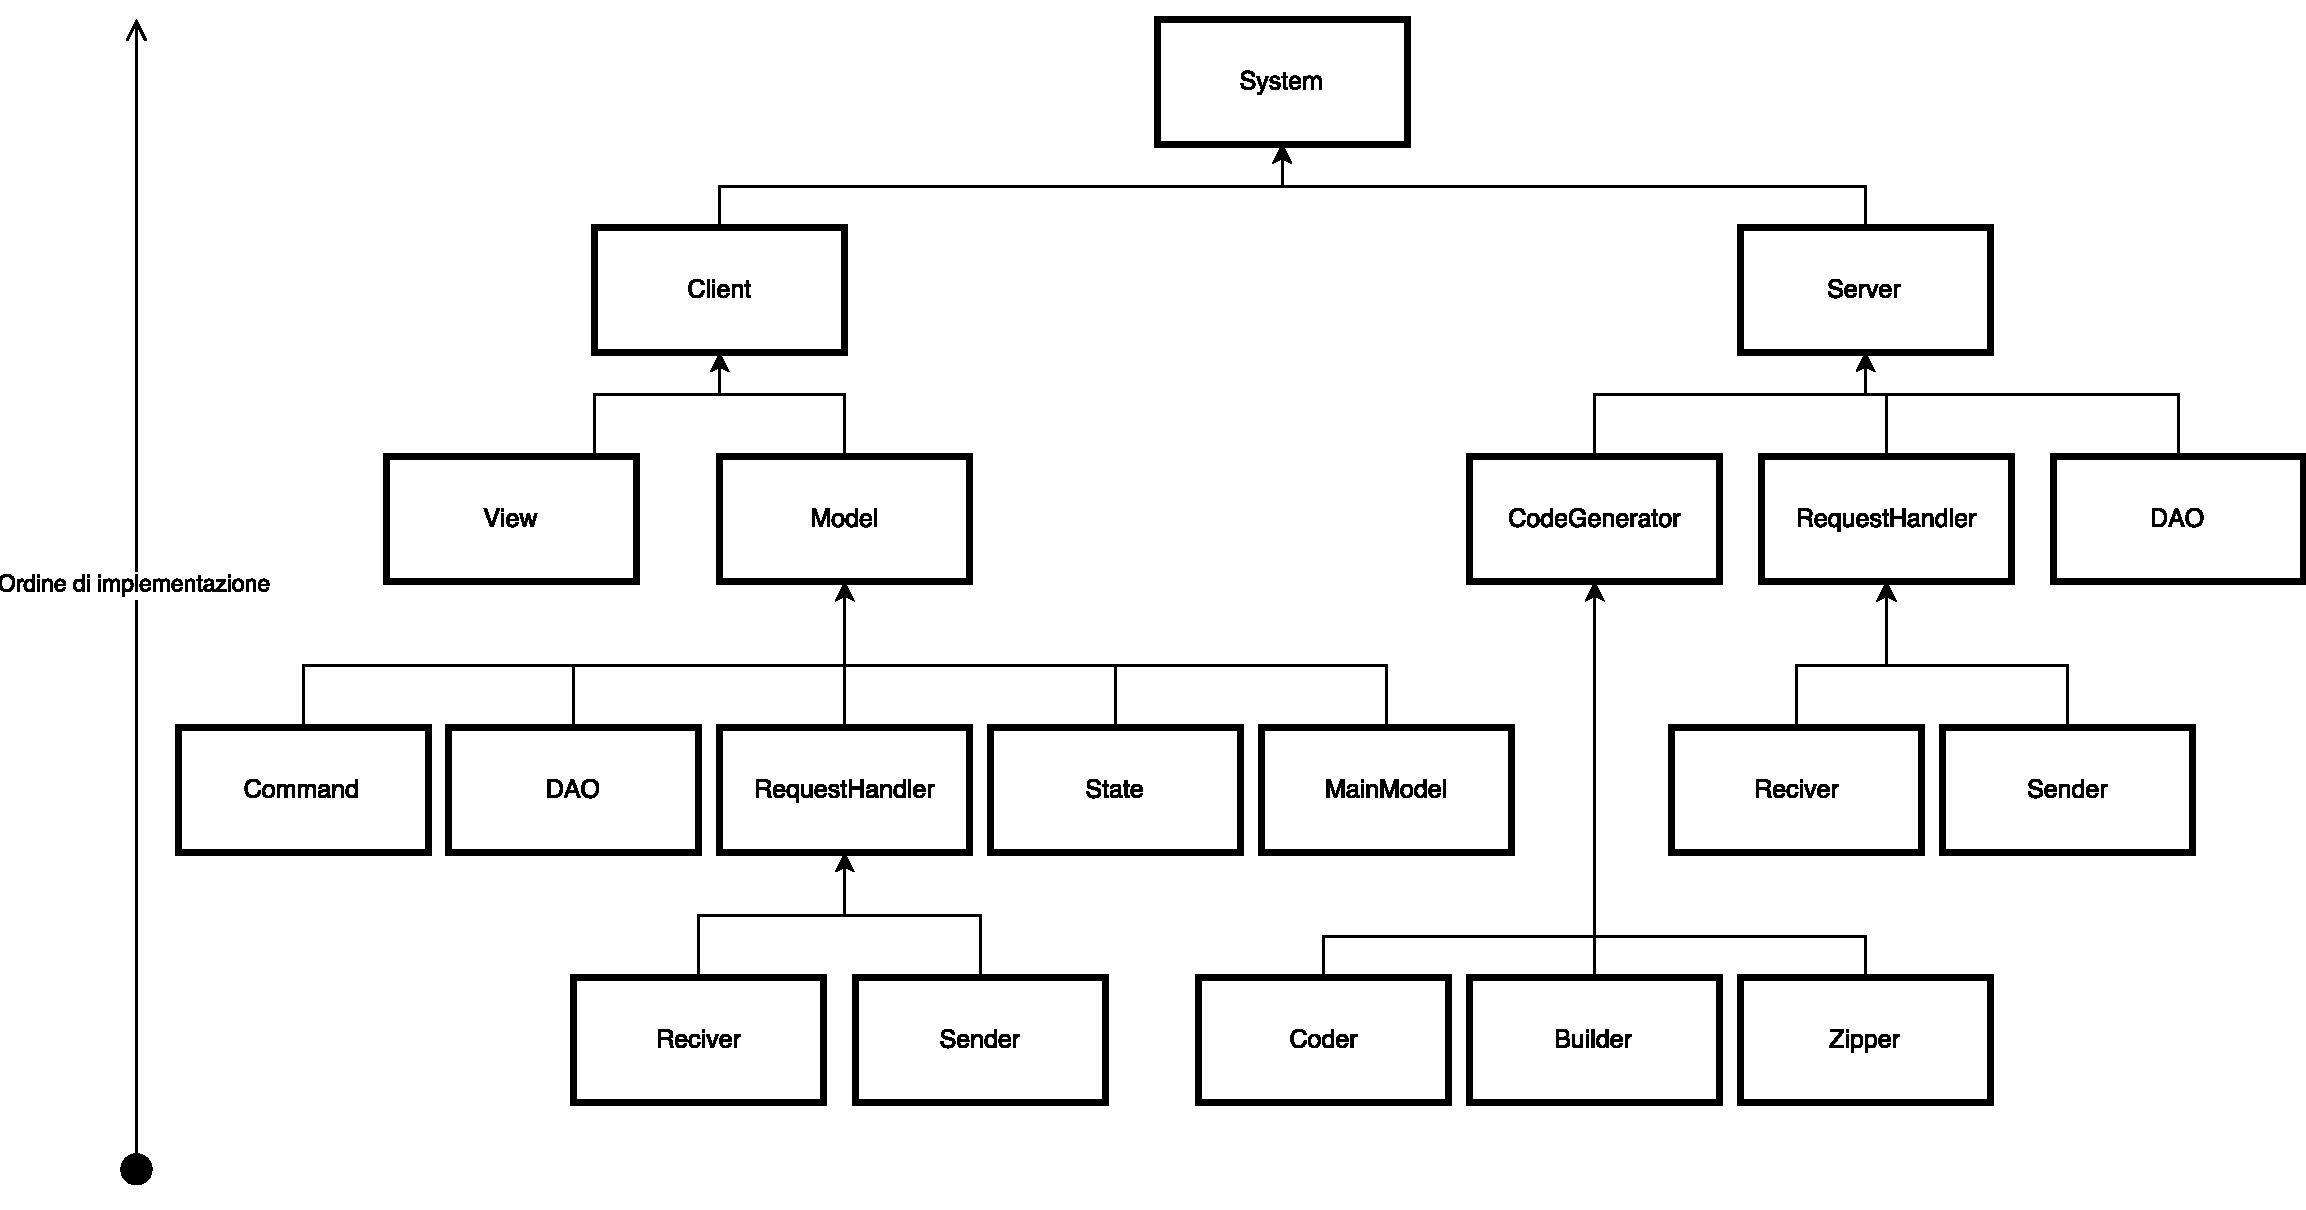
\includegraphics[scale=0.4]{Figures/Integrazione.pdf}
		\caption{Diagramma test di integrazione}\label{}
	\end{figure}
	
	
	% Sistema
	\subsubsection{Test TI1}
	\paragraph{Descrizione:}\hypertarget{TI1} Viene verificata l'integrazione finale per le componenti del sistema, in particolare tra Server e Client.
	\paragraph{Stato} Non implementato.
	\paragraph{Componente} SweDesigner.
	
	% Client
	\subsubsection{Test TI1.1}
	\paragraph{Descrizione:}\hypertarget{TI1.1} Viene verificata l'integrazione finale per le componenti del Client, in particolare tra  Model e View.
	\paragraph{Stato} Non implementato.
	\paragraph{Componente} SweDesigner::Client.
	
	% View
	\subsubsection{Test TI1.1.1}
	\paragraph{Descrizione:}\hypertarget{TI1.1.1} Viene verificato che il sistema gestisca correttamente le componenti della View in particolare l'integrazione tra la TitleBarView, la ToolBarView, l'AddressView, l'EditPanelView e il Paper.
	\paragraph{Stato} Non implementato.
	\paragraph{Componente} SweDesigner::Client::View.
	
	\subsubsection{Test TI1.1.2}
	\paragraph{Descrizione:}\hypertarget{TI1.1.2} Viene verificato che il sistema gestisca correttamente le componenti della View in particolare l'integrazione dei vari moduli con la libreria esterna \gl{JointJS}.
	\paragraph{Stato} Non implementato.
	\paragraph{Componente} SweDesigner::Client::View.
	
	% Model
	\subsubsection{Test TI1.1.3}
	\paragraph{Descrizione:}\hypertarget{TI1.1.3} Viene verificata l'integrazione per le componenti del Model, in particolare Command, Dao, RequestHendler, Main Model e State.
	\paragraph{Stato} Non implementato.
	\paragraph{Componente} SweDesigner::Client::Model.
	
	% Command
	\subsubsection{Test TI1.1.3.1}
	\paragraph{Descrizione:}\hypertarget{TI1.1.3.1} Viene verificato che il modulo Command gestisca correttamente i vari comandi impartiti dai moduli della View ai rispettivi moduli del Model.
	\paragraph{Stato} Non implementato.
	\paragraph{Componente} SweDesigner::Client::Model::Command.
	
	% Dao 1.1.2.2
	\subsubsection{Test TI1.1.3.2}
	\paragraph{Descrizione:}\hypertarget{TI1.1.3.2} Viene verificato che il DAO all'interno del Model carichi correttamente un progetto.
	\paragraph{Stato} Non implementato.
	\paragraph{Componente} SweDesigner::Client::Model::DAO.
	
	\subsubsection{Test TI1.1.3.3}
	\paragraph{Descrizione:}\hypertarget{TI1.1.3.3} Viene verificato che il DAO all'interno del Model salvi correttamente un progetto.
	\paragraph{Stato} Non implementato.
	\paragraph{Componente} SweDesigner::Client::Model::DAO.
	
	% RequestHandler 1.1.2.3
	\subsubsection{Test TI1.1.3.4}
	\paragraph{Descrizione:}\hypertarget{TI1.1.3.4} Viene verificata l'integrazione per le componenti del RequestHandler del Client, in particolare Sender e Receiver.
	\paragraph{Stato} Non implementato.
	\paragraph{Componente} SweDesigner::Client::Model::RequestHandler.
	
	% Sender 1.1.2.3.1
	\subsubsection{Test TI1.1.3.4.1}
	\paragraph{Descrizione:}\hypertarget{TI1.1.3.4.1} Viene verificato che il Sender all'interno del Client invii le richieste per bubble correttamente al Server.
	\paragraph{Stato} Non implementato.
	\paragraph{Componente} SweDesigner::Client::Model::RequestHandler::Sender.
	
	\subsubsection{Test TI1.1.3.4.2}
	\paragraph{Descrizione:}\hypertarget{TI1.1.3.4.2} Viene verificato che il Sender all'interno del Client invii  correttamente al Server le richieste per la creazione di codice a partire dal file \gl{JSON}.
	\paragraph{Stato} Non implementato.
	\paragraph{Componente} SweDesigner::Client::Model::RequestHandler::Sender.
	
	% Receiver 1.1.2.3.2
	\subsubsection{Test TI1.1.3.5}
	\paragraph{Descrizione:}\hypertarget{TI1.1.3.5} Viene verificato che il Receiver all'interno del Client riceva correttamente le bubble dal Server.
	\paragraph{Stato} Non implementato.
	\paragraph{Componente} SweDesigner::Client::Model::RequestHandler::Receiver.
	
	% MainModel 1.1.2.4
	\subsubsection{Test TI1.1.3.6}
	\paragraph{Descrizione:}\hypertarget{TI1.1.3.6} Viene verificata l'integrazione per il MainModel all'interno del Client con i vari moduli del Model collegati ai moduli della View, in particolare con il DiagramTree, la TitleBarModel, la ToolBarModel, l'AddressModel e l'EditPanelModel. 
	\paragraph{Stato} Non implementato.
	\paragraph{Componente} SweDesigner::Client::Model::MainModel.
	
	% Diagram 1.1.2.4.1
	\subsubsection{Test TI1.1.3.7}
	\paragraph{Descrizione:}\hypertarget{TI1.1.3.7} Viene verificata l'integrazione per il modulo Diagram all'interno del Client con il framework JointJS. 
	\paragraph{Stato} Non implementato.
	\paragraph{Componente} SweDesigner::Client::Model::Diagram.
	
	% State 1.2.3.5
	\subsubsection{Test TI1.1.3.8}
	\paragraph{Descrizione:}\hypertarget{TI1.1.3.8} Viene verificato che lo State del Client memorizzi correttamente la sequenza dei vari Command. 
	\paragraph{Stato} Non implementato.
	\paragraph{Componente} SweDesigner::Client::Model::State.
	
	% Server 1.2
	\subsubsection{Test TI1.2}
	\paragraph{Descrizione:}\hypertarget{TI1.2} Viene verificata l'integrazione per le componenti del Server, in particolare RequestHandler, DAO e CodeGenerator.
	\paragraph{Stato} Non implementato.
	\paragraph{Componente} SweDesigner::Server.
	
	% RequestHandler
	\subsubsection{Test TI1.2.1}
	\paragraph{Descrizione:}\hypertarget{TI1.2.1} Viene verificata l'integrazione per le componenti del RequestHandler del Server, in particolare Sender e Receiver.
	\paragraph{Stato} Non implementato.
	\paragraph{Componente} SweDesigner::Server::RequestHandler.
	
	% Sender
	\subsubsection{Test TI1.2.1.1}
	\paragraph{Descrizione:}\hypertarget{TI1.2.1.1} Viene verificato che il Sender all'interno del Server invii le bubble correttamente al Client.
	\paragraph{Stato} Non implementato.
	\paragraph{Componente} SweDesigner::Server::RequestHandler::Sender.
	
	\subsubsection{Test TI1.2.1.2}
	\paragraph{Descrizione:}\hypertarget{TI1.2.1.2} Viene verificato che il Sender all'interno del Server invii correttamente al Client il file .zip contenente il codice generato.
	\paragraph{Stato} Non implementato.
	\paragraph{Componente} SweDesigner::Server::RequestHandler::Sender.
	
	% Receiver 1.2.1.2
	\subsubsection{Test TI1.2.1.3}
	\paragraph{Descrizione:}\hypertarget{TI1.2.1.3} Viene verificato che il Receiver all'interno del Server riceva correttamente dal Client il file JSON necessario alla generazione del codice.
	\paragraph{Stato} Non implementato.
	\paragraph{Componente} SweDesigner::Server::RequestHandler::Receiver.
	
	% Dao 
	\subsubsection{Test TI1.2.2}
	\paragraph{Descrizione:}\hypertarget{TI1.2.2} Viene verificato che il DAO all'interno del Server restituisca correttamente una bubble.
	\paragraph{Stato} Non implementato.
	\paragraph{Componente} SweDesigner::Server::DAO.
	
	\subsubsection{Test TI1.2.3}
	\paragraph{Descrizione:}\hypertarget{TI1.2.3} Viene verificato che il DAO all'interno del Server salvi correttamente una bubble.
	\paragraph{Stato} Non implementato.
	\paragraph{Componente} SweDesigner::Server::DAO.
	
	%CodeGenerator
	\subsubsection{Test TI1.2.4}
	\paragraph{Descrizione:}\hypertarget{TI1.2.4} Viene verificata l'integrazione per le componenti del CodeGenerator del Server, in particolare Coder, Builder e Zipper.
	\paragraph{Stato} Non implementato.
	\paragraph{Componente} SweDesigner::Server::CodeGenerator.
	
	% JSON.Parse()
	\subsubsection{Test TI1.2.5}
	\paragraph{Descrizione:}\hypertarget{TI1.2.5} Viene verificata l'integrazione per le componenti del CodeGenerator del Server con il metodo Javascript JSON.parse().
	\paragraph{Stato} Non implementato.
	\paragraph{Componente} SweDesigner::Server::CodeGenerator.
	
	% Coder
	\subsubsection{Test TI1.2.6}
	\paragraph{Descrizione:}\hypertarget{TI1.2.6} Viene verificato che il Coder all'interno del Server costruisca correttamente i file a partire dagli oggetti costruiti tramite il metodo JSON.parse().
	\paragraph{Stato} Non implementato.
	\paragraph{Componente} SweDesigner::Server::CodeGenerator::Coder.
	
	% Builder
	\subsubsection{Test TI1.2.7}
	\paragraph{Descrizione:}\hypertarget{TI1.2.7} Viene verificato che il Builder all'interno del Server organizzi i file in cartelle seguendo le istruzioni contenute nel file JSON inviato dal Client.
	\paragraph{Stato} Non implementato.
	\paragraph{Componente} SweDesigner::Server::CodeGenerator::Builder.
	
	% JSZip
	\subsubsection{Test TI1.2.8}
	\paragraph{Descrizione:}\hypertarget{TI1.2.8} Viene verificato che lo Zipper del Server crei correttamente il file .zip a partire da file sorgenti e cartelle generati.
	\paragraph{Stato} Non implementato.
	\paragraph{Componente} SweDesigner::Server::CodeGenerator::Zipper.
	
	\newpage
	\subsection{Tracciamento test di integrazione}
	\normalsize
	\begin{longtable}{|c|l|}
		\hline
		\textbf{Test di integrazione} & \textbf{Componente}\\
		\hline
		\endhead
		\hyperlink{TI1}{TI1} & SweDesigner \\
		\hline
		\hyperlink{TI1.1}{TI1.1} & SweDesigner::Client \\
		\hline
		\hyperlink{TI1.1.1}{TI1.1.1} & SweDesigner::Client::View \\
		\hline
		\hyperlink{TI1.1.2}{TI1.1.2} & SweDesigner::Client::View \\
		\hline
		\hyperlink{TI1.1.3}{TI1.1.3} & SweDesigner::Client::Model \\
		\hline
		\hyperlink{TI1.1.3.1}{TI1.1.3.1} & SweDesigner::Client::Model::Command \\
		\hline
		\hyperlink{TI1.1.3.2}{TI1.1.3.2} & SweDesigner::Client::Model::DAO \\
		\hline
		\hyperlink{TI1.1.3.3}{TI1.1.3.3} & SweDesigner::Client::Model::DAO \\
		\hline
		\hyperlink{TI1.1.3.4}{TI1.1.3.4} & SweDesigner::Client::Model::RequestHandler \\
		\hline
		\hyperlink{TI1.1.3.4.1}{TI1.1.3.4.1} & SweDesigner::Client::Model::RequestHandler::Sender \\
		\hline
		\hyperlink{TI1.1.3.4.2}{TI1.1.3.4.2} & SweDesigner::Client::Model::RequestHandler::Sender \\
		\hline
		\hyperlink{TI1.1.3.5}{TI1.1.3.5} & SweDesigner::Client::Model::RequestHandler::Receiver \\
		\hline
		\hyperlink{TI1.1.3.6}{TI1.1.3.6} & SweDesigner::Client::Model::MainModel \\
		\hline
		\hyperlink{TI1.1.3.7}{TI1.1.3.7} & SweDesigner::Client::Model::Diagram \\
		\hline
		\hyperlink{TI1.1.3.8}{TI1.1.3.8} & SweDesigner::Client::Model::State \\
		\hline
		\hyperlink{TI1.2}{TI1.2} & SweDesigner::Server \\
		\hline
		\hyperlink{TI1.2.1}{TI1.2.1} & SweDesigner::Server::RequestHandler \\
		\hline
		\hyperlink{TI1.2.1.1}{TI1.2.1.1} & SweDesigner::Server::RequestHandler::Sender \\
		\hline
		\hyperlink{TI1.2.1.2}{TI1.2.1.2} & SweDesigner::Server::RequestHandler::Sender \\
		\hline
		\hyperlink{TI1.2.1.3}{TI1.2.1.3} & SweDesigner::Server::RequestHandler::Receiver \\
		\hline
		\hyperlink{TI1.2.2}{TI1.2.2} & SweDesigner::Server::DAO \\
		\hline
		\hyperlink{TI1.2.3}{TI1.2.3} & SweDesigner::Server::DAO \\
		\hline
		\hyperlink{TI1.2.4}{TI1.2.4} & SweDesigner::Server \\
		\hline
		\hyperlink{TI1.2.5}{TI1.2.5} & SweDesigner::Server::CodeGenerator \\
		\hline
		\hyperlink{TI1.2.6}{TI1.2.6} & SweDesigner::Server::CodeGenerator::Coder \\
		\hline
		\hyperlink{TI1.2.7}{TI1.2.7} & SweDesigner::Server::CodeGenerator::Builder \\
		\hline
		\hyperlink{TI1.2.8}{TI1.2.8} & SweDesigner::Server::CodeGenerator::Zipper \\
		\hline
		\caption[Tracciamento test di integrazione]{Tracciamento test di integrazione}
		\label{tabella:TracciamentoTestIntegrazione}
	\end{longtable}
\end{document} 